\documentclass{report}


\usepackage{amsmath} % Better matrix environment
\usepackage{amssymb}
\usepackage[inline]{enumitem} % inline numbering and resume numbering
\usepackage{etoolbox} % If conditions
\usepackage{graphicx}
\usepackage{listings} % for code
\usepackage{hyperref}
\usepackage{caption}
\usepackage{pgfplotstable}
\pgfplotsset{compat=1.10}
\usepackage{subcaption}
\usepackage{svg}
\usepackage{tikz}
\usepackage{tikz-qtree,tikz-qtree-compat} % Trees
\usepackage{xkeyval}

\pdfoptionpdfminorversion=5

% Squiggly lines
\usetikzlibrary{decorations.pathmorphing}


% Node shapes
\usetikzlibrary{shapes,decorations}

% Coordinate calculation
\usetikzlibrary{calc}

% For charts
\usetikzlibrary{patterns}

\newcommand{\VertexSet}{V}
\newcommand{\CellSet}{C}

\newcommand{\Visited}{V_{visited}}

% Adjacency relation
\newcommand{\AdjVV}{Adj_{\VertexSet\VertexSet}}

% Cardinality of
\newcommand{\card}[1]{\left\vert{#1}\right\vert}

% powerset of
\newcommand{\powerset}[1]{\mathcal P \left({#1}\right)}


% Tikz function: compute absolute position
% row, delta-sy, y-offset
\newcommand{\rctoxy}[3][3=0]{#1*#2 + #3}



% Line that can go anywhere, structured region or outside
\tikzset{%
    anywhere/.style={
		decorate,
		decoration={
		    snake,
		    segment length=4,
		    amplitude=.9,post=lineto,
		    post length=2pt
		}
	}
}

% Line that can only go outside the structured region
\tikzset{outside/.style={dotted}}


% Ellipsis
\tikzset{ellipsis/.style={loosely dotted}}

% Structured
\tikzset{structured/.style={}}


%% Node labelling functions

% row, col, rowoffset, coloffset
\newcommand{\plainlabelnode}[4]{
\pgfmathtruncatemacro{\rowlabel}{#1+#3}\pgfmathtruncatemacro{\collabel}{#2+#4}$n_{\rowlabel,\collabel}$}

% row, col, rowoffset, coloffset, column-variable
\newcommand{\varcollabelnode}[5]{
\pgfmathtruncatemacro{\row}{#1+#3}\pgfmathtruncatemacro{\col}{#2+#4}\pgfmathtruncatemacro{\colzero}{\col-1}\newcommand{\collabel}{\ifnumcomp{\colzero}{=}{0}{#5}{\ifnumcomp{\colzero}{>}{0}{#5+\colzero}{#5\colzero}}}$n_{\row,\collabel}$}

% row, col, rowoffset, coloffset, row-variable
\newcommand{\varrowlabelnode}[5]{\pgfmathtruncatemacro{\row}{#1+#3}\pgfmathtruncatemacro{\rowzero}{\row-1}\pgfmathtruncatemacro{\col}{#2+#4}\newcommand{\rowlabel}{\ifnumcomp{\rowzero}{=}{0}{#5}{\ifnumcomp{\rowzero}{>}{0}{#5+\rowzero}{#5\rowzero}}}$n_{\rowlabel,\col}$}


% row, col, rowoffset, coloffset, row-variable, col-variable
\newcommand{\varlabelnode}[6]{\pgfmathtruncatemacro{\row}{#1+#3}\pgfmathtruncatemacro{\rowzero}{\row-1}\pgfmathtruncatemacro{\col}{#2+#4}\pgfmathtruncatemacro{\colzero}{\col-1}\newcommand{\rowlabel}{\ifnumcomp{\rowzero}{=}{0}{#5}{\ifnumcomp{\rowzero}{>}{0}{#5+\rowzero}{#5\rowzero}}}\newcommand{\collabel}{\ifnumcomp{\colzero}{=}{0}{#6}{\ifnumcomp{\colzero}{>}{0}{#6+\colzero}{#6\colzero}}}$n_{\rowlabel,\collabel}$}



\pgfkeys{/tikz/.cd,% to set the path
  rows/.get=\krows,
  rows/.store in=\krows,
  cols/.get=\kcols,
  cols/.store in=\kcols,
  rowoffset/.initial=0,
  rowoffset/.get=\krowoffset,
  rowoffset/.store in=\krowoffset,
  coloffset/.initial=0,
  coloffset/.get=\kcoloffset,
  coloffset/.store in=\kcoloffset,
  labeler/.get=\klabeler,
  labeler/.store in=\klabeler,
  labelerA/.get=\klabelerA,
  labelerA/.store in=\klabelerA,
  labelerB/.get=\klabelerB,
  labelerB/.store in=\klabelerB,
  labelerC/.get=\klabelerC,
  labelerC/.store in=\klabelerC,
  labelerD/.get=\klabelerD,
  labelerD/.store in=\klabelerD,
  northborder/.initial=outside,
  northborder/.get=\knorthborder,
  northborder/.store in=\knorthborder,
  southborder/.initial=outside,
  southborder/.get=\ksouthborder,
  southborder/.store in=\ksouthborder,
  eastborder/.initial=outside,
  eastborder/.get=\keastborder,
  eastborder/.store in=\keastborder,
  westborder/.initial=outside,
  westborder/.get=\kwestborder,
  westborder/.store in=\kwestborder,
}

%% Draws a grid - num rows, num cols, row offset, col offset
\newcommand{\drawgrid}[1]{{
     \tikzset{#1}


	\newcommand{\maxrows}{\krows}
	\newcommand{\maxcols}{\kcols}
	\newcommand{\rowoffset}{\krowoffset}
	\newcommand{\coloffset}{\kcoloffset}
	% Argument is a function: r,c -> node label
	\newcommand{\labeler}{\klabeler}

	\foreach \row in {1,...,\maxrows} {
		\pgfmathsetmacro{\ypos}{-2 * \row + \rowoffset}
		\pgfmathtruncatemacro{\prevrow}{\row - 1}

		\foreach \col in {1,...,\maxcols} {
			\pgfmathsetmacro{\xpos}{2 * \col + \coloffset}
			\pgfmathtruncatemacro{\prevcol}{\col - 1}
			\newcommand{\thisnode}{(n \row \space \col)}

			% Get node label
			\ifstrempty{\klabelerA}{
				\newcommand{\nodelabel}{\labeler{\row}{\col}}
			}
			\ifstrempty{\klabelerB} {
				\newcommand{\nodelabel}{\labeler{\row}{\col}{\klabelerA}}
			}
			\ifstrempty{\klabelerC} {
				\newcommand{\nodelabel}{\labeler{\row}{\col}{\klabelerA}{\klabelerB}}
			}
			\ifstrempty{\klabelerD} {
				\newcommand{\nodelabel}{\labeler{\row}{\col}{\klabelerA}{\klabelerB}{\klabelerC}}
			}
			{
				\newcommand{\nodelabel}{\labeler{\row}{\col}{\klabelerA}{\klabelerB}{\klabelerC}{\klabelerD}}
			}
			% Create node
			\node (n \row \space \col) at (\xpos,\ypos) {\nodelabel};

			% Line from node to the previous horizontal node
			\ifnumcomp{\col}{>}{1} {
				\draw (n \row \space \prevcol) -- \thisnode;
			}

			% Line from node to the previous vertical node
			\ifnumcomp{\row}{>}{1} {
				\draw (n \prevrow \space \col) -- \thisnode;
			}


			% West border lines
			\ifnumcomp{\col}{=}{1} {
				\draw[\kwestborder] \thisnode -- (\xpos-1, \ypos);
			}
			% East border lines
			\ifnumcomp{\col}{=}{\maxcols} {
				\draw[\keastborder] (\xpos+1, \ypos) -- \thisnode;
			}

			% North border lines
			\ifnumcomp{\row}{=}{1} {
				\draw[\knorthborder] \thisnode -- (\xpos, \ypos+1);
			}
			% South border lines
			\ifnumcomp{\row}{=}{\maxrows} {
				\draw[\ksouthborder] (\xpos, \ypos-1) -- \thisnode;
			}
		}
	}
}}
\pgfkeys{/tikz/.cd,% to set the path
  num/.get=\knum,
  num/.store in=\knum,
  rowoffset/.initial=0,
  rowoffset/.get=\krowoffset,
  rowoffset/.store in=\krowoffset,
  coloffset/.initial=0,
  coloffset/.get=\kcoloffset,
  coloffset/.store in=\kcoloffset,
}


%% Draws a row of vertical ellipses - num cols, row offset, col offset
\newcommand{\drawellipsisrow}[1]{{
	\tikzset{#1}

	\newcommand{\numellipses}{\knum}
	\newcommand{\rowoffset}{\krowoffset}
	\newcommand{\coloffset}{\kcoloffset}

	\foreach \col in {1,...,\numellipses} {
		\pgfmathsetmacro{\xpos}{2 * \col + \coloffset}
		\pgfmathsetmacro{\ypos}{\rowoffset}

		\draw[ellipsis] (\xpos, \ypos) -- (\xpos, \ypos-1);
	}
}}



\pgfkeys{/tikz/.cd,% to set the path
  num/.get=\knum,
  num/.store in=\knum,
  rowoffset/.initial=0,
  rowoffset/.get=\krowoffset,
  rowoffset/.store in=\krowoffset,
  coloffset/.initial=0,
  coloffset/.get=\kcoloffset,
  coloffset/.store in=\kcoloffset,
}


%% Draws a column of horizontal ellipses - num rows, row offset, col offset
\newcommand{\drawellipsiscol}[1]{{
	\tikzset{#1}

	\newcommand{\numellipses}{\knum}
	\newcommand{\rowoffset}{\krowoffset}
	\newcommand{\coloffset}{\kcoloffset}

	\foreach \row in {1,...,\numellipses} {
		\pgfmathsetmacro{\xpos}{\coloffset}
		\pgfmathsetmacro{\ypos}{-2 * \row + \rowoffset}

		\draw[ellipsis] (\xpos, \ypos) -- (\xpos+1, \ypos);
	}
}}


\begin{document}

\chapter{Introduction}
Scientific computing is a large research branch touching on various areas in the scientific community as well as in various industries. An integral part of it is concerned with algorithms and techniques which operate on a mesh representation of a model, typically modelling physical phenomena such as the motion of fluids. SEE
% [Flow simulation and high performance computing, 1996a T. Tezduyar, http://www.tafsm.org/PUB_PRE/jALL/j63-CM96.pdf]
. SEE
% [http://www.sv.vt.edu/classes/MSE2094_NoteBook/97ClassProj/num/widas/history.html]
for a good introduction on finite element analysis.


Various methods of representing meshes exist, including X, Y, and Z
% [http://en.wikipedia.org/wiki/Polygon_mesh#Representations]
. Representations typically rely on encoding some form of explicitly-defined mapping between mesh elements. This can be represented straightforwardly as a flat array, with the array indices representing elements in the source set, and each value being one or more values representing one or more elements in the destination/target set. We focus our attention to the case where the number of target elements mapped to from each source element is constant. Such a map is known as a constant-arity map.

Consider for instance a quadrilateral mesh with two element sets \texttt{C} and \texttt{V}, representing the set of cells and vertices, respectively.
We can define a dat of coordinates, which associates the set each vertex $v \in V$ with a coordinate pair $(x_v, y_v)$, representing its position in 2D space.

We can then define an adjacency map (of constant arity 4) from cells to vertices:

\texttt{$C \rightarrow Node^4$}

Now consider an operation over this mesh, which performs a computation for each cell $c \in C$ as a function of its adjacent nodes ${n | n \in Map[c]}$, for instance computing the area of the cell. In particular consider the chain of memory access indirections and the resulting memory access patterns:

%
%             |   |             |   |
%             |   |  /----n3--->|   | -> (x_1, y_1)
%             |   | /           |   |
% cell_id ->  |   |/------n1--->|   | -> (x_4, y_4)
%             |   |\            |   |
%             |   | \-----n4--->|   | -> (x_5, y_5)
%             |   |  \          |   |
%             |   |   \---n2--->|   | -> (x_12, y_12)
%             |   |             |   |
%             |   |             |   |
%             |   |             |   |
%           cell2nodes         node2coordinate

Notice that proximate (or indeed adjacent) nodes in the mesh need not exhibit a uniform memory access pattern. This is detrimental to performance for various reasons.
1. They do not exhibit spatial locality, a property which most modern CPU caches bank on to attain higher performance in IO bound applications, which may manifest through decisions regarding cache replacement strategies or data pre-fetching.
2. Looking up addresses, as opposed to computing them directly, will typically prohibit or limit the scope of compiler-performed optimizations, not least vectorizations.

Numerous strategies have been devoted to deal with this problem, notably applying a space filling curve to obtain a more favourable numbering, with closer elements tending to have closer numberings. While the space filling curve most certainly improves cache locality, it does not make use more obvious structure that may exist. A mesh that is irregular and unstructured on the whole may contain subregions of high regularity and uniform structure, whose regularity/uniformity may be locally exploitable in a more direct manner, for potentially higher gain!


We present Crystal mesh, a group of algorithms for \emph{extracting} regions of regularity in a mesh, reorganizing the mesh to \emph{expose} said structure in order to enable efficient \emph{exploitation}.
In particular, we present and evaluate an implementation for extracting and exposing structure in quadrilateral meshes on various examples, and evaluate a 33\% performance improvement achieved by exploiting the structure on the airfoil computation.


\chapter{Background}
Before continuing further, we introduce briefly the main notions required to appreciate this work.

\section{The mathematical mesh model}

Meshes often model physical objects and phenomena. This is typically achieved through the discretization of a continuous model, such as the surface or volume of an object, in order to approximate its physical properties to a desired degree of precision.
\par

The mesh model consists of a hierarchy of elements, which may include a subset the following:
\begin{itemize}
\item Polyhedra such as cubes or tetrahedrons
\item Polygons \emph{(also referred to as cells or faces)} such as triangles and quadrilaterals
\item Edges
\item Vertices \emph{(also referred to as nodes)}
\end{itemize}

\includesvg[width=\imagewidth, svgpath=images/background/]{mesh-elements}

Each element in the above hierarchy is built-up from those below it. Thus, a polyhedron is assimilated by a set of polygons, a polygon is composed by a set of edges, and an edge joins two vertices.


\subsection{Geometry vs topology}
There is a key distinction to make between the geometric and topological properties of a mesh.

Since meshes model a physical reality, the elements of a mesh may be spatially embedded: vertices are associated with points in space, and edges are formed as segments joining their two vertices. This affects \emph{geometric} properties of the mesh, such as its surface area or volume.

On the other hand, the hierarchy of elements described above induces a mesh topology. This describes the connectedness of the mesh, that is to say how elements relate to one another. For instance, we may describe two vertices sharing an edge as \emph{adjacent}, or two cells being sharing an edge as being \emph{incident} on that edge.
\par
In this work we concern ourselves solely with the topological structure of meshes, treating its geometry as arbitrary data that is associated with its respective elements (the position of a vertex for instance). Figure~\ref{fig:same-topology} illustrates the difference between the two concepts.

\begin{figure}
    \includesvg[width=\imagewidth, svgpath=images/background/]{same-topology}
    \caption{Despite having completely different geometric shapes and properties, the two meshes are topologically equivalent. The labels indicate corresponding vertices.}
    \label{fig:same-topology}
\end{figure}




\subsection{Manifold meshes}
A mesh is a manifold if the following properties hold:
\begin{enumerate}
\item All edges are adjacent to either one or two faces.

\item All faces meeting at a given vertex must form either an open or a closed fan around that vertex (Figure~\ref{fig:open-closed-fans}).
\end{enumerate}

% Open and closed fans
\begin{figure}
    \sidebyside
        {\includesvg[width=\imagewidth, svgpath=images/background/]{closed-fan}
        \caption{A closed fan}}
        {\includesvg[width=\imagewidth, svgpath=images/background/]{open-fan}
        \caption{An open fan}}
    \caption{}
    \label{fig:open-closed-fans}
\end{figure}

Figure~\ref{fig:non-manifolds} demonstrates examples of non-manifold meshes. In this work we consider manifold meshes exclusively, and future mentions of `mesh' shall implicitly refer to manifold meshes.

% Non-manifolds
\begin{figure}
    \sidebysidefour
    {\includesvg[width=\textwidth, svgpath=images/background/]{bad-fan}
        \caption{Faces incident on a vertex which do not form a continuous fan}}
    {\includesvg[width=\textwidth, svgpath=images/background/]{bad-fan2}
        \caption{An extra face that breaks off from the otherwise closed fan}}
    {\includesvg[width=\textwidth, svgpath=images/background/]{bad-multi-edge}
        \caption{More than two faces incident on a single edge}}
    {\includesvg[width=\textwidth, svgpath=images/background/]{bad-no-edge}
        \caption{An edge with no incident faces}}

    \caption{Examples of non-manifold meshes.}
    \label{fig:non-manifolds}
\end{figure}





\section{The mesh data structure}

We describe how a mesh model is manifest at the data structure level. There are three general component types can be identified:
\begin{itemize}
\item Entity sets
\item Associative data
\item Relations between two entity sets
\end{itemize}

In the following sections, the examples shall refer to the mesh depicted in figure~\ref{fig:example-mesh}.

\begin{figure}
    \includesvg[width=\textwidth, svgpath=images/background/]{mesh-data-structure}
    \caption{Example mesh with labelled elements.}
    \label{fig:example-mesh}
\end{figure}


\subsection{Entity sets}
Each set represents a certain type of entity in the mesh, such as vertices or cells. Each element in a set is associated with a unique identifier. Integers are a common choice as an identifier for a couple of reasons:
\begin{itemize}
\item They need not be enumerated explicitly. All we need is the set cardinality and a starting index.
\item They are convenient for direct-indexed array accesses, as well as for more general indexing methods.
\end{itemize}

See figure~\ref{fig:entity-sets} for examples.

\begin{figure}
    \includesvg[width=\textwidth, svgpath=images/background/]{entity-sets}
    \caption{The entity sets of the mesh in figure~\ref{fig:example-mesh}. These are (from left to right) the vertices, edges, and cells.}
    \label{fig:entity-sets}
\end{figure}


\subsection{Associative data}
Arbitrary data which is associated with elements of a particular entity set. For instance, spatial coordinates associated with each vertex. A typical representation is a flat array indexed by element identifier.
This is the data over which we perform our computations and ultimately care about. Everything else is incidental.
See figure~\ref{fig:associative-data} for an example.

\begin{figure}
    \includesvg[width=\textwidth, svgpath=images/background/]{associative-data}
    \caption{Coordinate data associated with the vertices of the mesh in figure~\ref{fig:example-mesh}.}
    \label{fig:associative-data}
\end{figure}


\subsection{Relation maps between two entity sets}
Entity sets may have relations defined between them, a mapping from an element in a source set to one or more corresponding elements in the destination set. For instance, we may have an adjacency relation from the vertex set to itself, or an inclusion relation from the cell set to the vertex set.
In a general unstructured mesh these relations must be explicitly stored, typically as an array indexed by the source element's identifier.
See figure~\ref{fig:relation} for an example.

\begin{figure}
    \includesvg[width=\textwidth, svgpath=images/background/]{relation}
    \caption{Inclusion relation from cells to vertices, as depicted in the mesh of figure~\ref{fig:example-mesh}.}
    \label{fig:relation}
\end{figure}




\section{The core-computation contract}
Given a mesh model and its underlying representation, computation logic provided by an external user is to be executed. We refer to this as the \emph{core-computation} so as to disambiguate it from other incidental processing, such as structure detection.
Our contract to the user is described in what follows.

\subsection{Given: operating set}
We are given an entity set over which to operate, for example the set of edges or the set of cells. We refer to this entity set as the \emph{operating set}. The core-computation consists of executing a computation for each element of the operating set. This is analogous to the \emph{map} phase of the MapReduce programming model~\cite{dean2008mapreduce}, though we restrict our usage of the term \emph{map} to refer to relation maps.

\subsection{Given: relation-map tree}
We are given a tree structure defining which relation maps to use and how to access them. This is best explained through an example, illustrated in figure~\ref{fig:relation-tree}. The core-computation will, for each element in the operating set, gather all indexing variables as described by the relation-map tree.


\begin{figure}
    %% Key icon
    \newcommand{\keyicon}{\includesvg[width=6pt, svgpath=images/background/]{key}}

    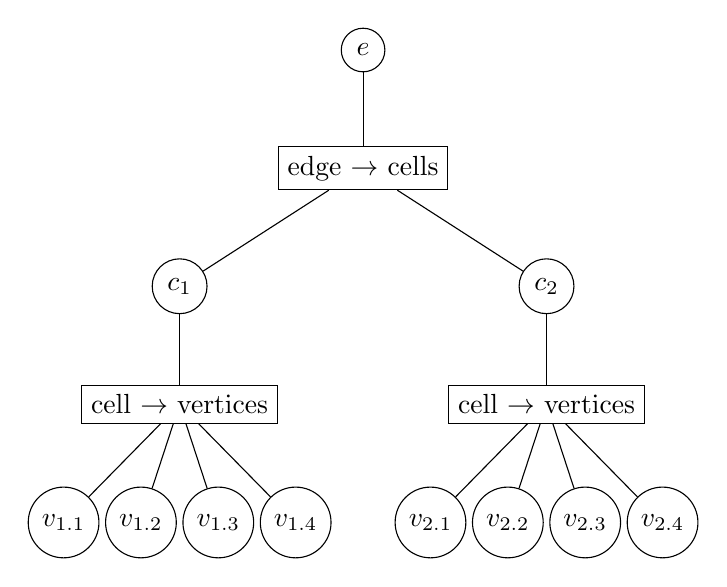
\begin{tikzpicture}[every tree node/.style={draw,circle},
        level distance=1.5cm,
        edge from parent path={(\tikzparentnode) -- (\tikzchildnode)}]

    \tikzset{level 2/.style={sibling distance=0.8cm}}

    \Tree
    [.{$e$}
        \edge node[auto=right] {\keyicon};
        [.\node[rectangle] {edge $\rightarrow$ cells};
            [.{$c_1$}
                \edge node[auto=right] {\keyicon};
                [.\node[rectangle] {cell $\rightarrow$ vertices};
                    [.$v_{1.1}$ ]
                    [.$v_{1.2}$ ]
                    [.$v_{1.3}$ ]
                    [.$v_{1.4}$ ]
                ]
            ]
            [.{$c_2$}
                \edge node[auto=right] {\keyicon};
                [.\node[rectangle] {cell $\rightarrow$ vertices};
                    [.$v_{2.1}$ ]
                    [.$v_{2.2}$ ]
                    [.$v_{2.3}$ ]
                    [.$v_{2.4}$ ]
                ]
            ]
        ]
    ]
    \end{tikzpicture}
    \caption{
    In this example, we consider a core-computation operating over the edge set, with $e$ being the indexing variable into the edge set.
    The edge $\rightarrow$ cells map is indexed by $e$ to obtain the the two cells $c_1$ and $c_2$ incident on the edge $e$. The cell $\rightarrow$ vertices map is then indexed by both $c_1$ and $c_2$ to obtain their respective vertices. The key symbol denotes indexing into the map below, using the indexing variable above.
    }
    \label{fig:relation-tree}
\end{figure}


\subsection{Given: kernel function}
\label{subsec:given-kernel-function}
We are given a kernel function specifying the computation logic, which is applied to each element in the operating set. It takes as arguments all gathered indexing variables, including that of the current element, and it has read and write access to the mesh's associated data. The access pattern of a kernel function is similar to that of a stencil computation, as defined by~\cite{tang2011pochoir}:
\begin{quote}
A stencil computation repeatedly updates each point of a d-dimensional grid as a function of itself and its near neighbours.
\end{quote}
As we define it, however, kernel functions are in fact more general than a stencil computation, as they access neighbouring elements across different operating sets.


The kernel function is applied to the operating set elements in no particular order; the indexing variables, however, are passed to the kernel in some known order, typically in the order stored in the relation-map.


\subsection{Expected operation}
Given all the above, a core-computation is then performed as follows:
\begin{enumerate}
\item Iterate over the elements of the operating set, in no particular order.
\item For each element iterated over:
    \begin{enumerate}
    \item Gather any indexing variables as defined by the relation-map tree. This may involve indexing variables obtained through a chain of relation-maps.
    \item Call the kernel function, passing the gathered indexing variables in some known order. The kernel function may access any associative data using these indexing variables.
    \end{enumerate}
\end{enumerate}



\section{Background on airfoils}
%% TODO CROSS REFERNCE to benchmarks
While not strictly needed for understanding our work, we nonetheless describe briefly airfoils and their function to offer a broader context. Much of this section was adapted from~\cite{abbott2012theory}, \cite{kuethe1986foundations} and~\cite{boeing2014airfoil}. Our description is nonetheless undoubtedly an overly simplistic one, and we would recommend that the aforementioned literature be sought for a fuller picture.

An airplane achieves flight by creating a lower air pressure over the wing (\emph{the upper surface}) whilst maintaining a higher air pressure below the wing (\emph{the lower surface}). The exact way in which this is achieved is characteristic of the wing shape as well as other factors. The pressure differential causes air in the lower surface to push towards the upper surface, creating a lift force. If the lift force is sufficient to counteract the gravitational force, the airplane flies.

An airfoil is the two-dimensional cross-section \emph{shape} of a wing. They are used to model the hydrodynamics (fluid motion) surrounding a particular wing shape in different contexts, including the velocity and angle of motion (known as the \emph{angle of attack}). Figure~\ref{fig:airfoil-crosscut} shows how the cross-section is taken, as well as the modelled air flow.

\begin{figure}
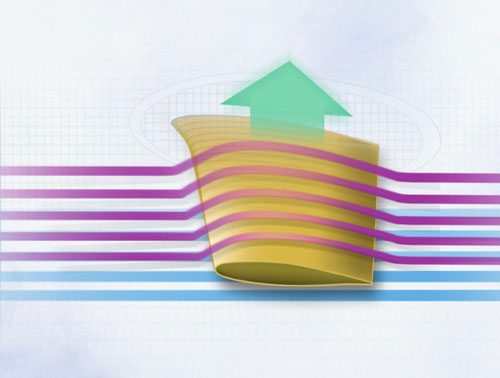
\includegraphics[width=\imagewidth]{images/background/airfoil_crosscut.jpg}
    \caption{The cross-section used to obtain the airfoil shape. Incoming air flow is split between the upper surface (purple) and the lower surface (blue). The image was obtained from~\cite{boeing2014airfoil}.}
    \label{fig:airfoil-crosscut}
\end{figure}


In 1929, the National Advisory Committee for Aeronautics (NACA) began to study various airfoils. They developed families of airfoil constructions parametrized by various geometric variables, depicted in figure~\ref{fig:airfoil-geometry}. We use specific instantiations of these airfoil families as benchmarks for Crystal.

\begin{figure}
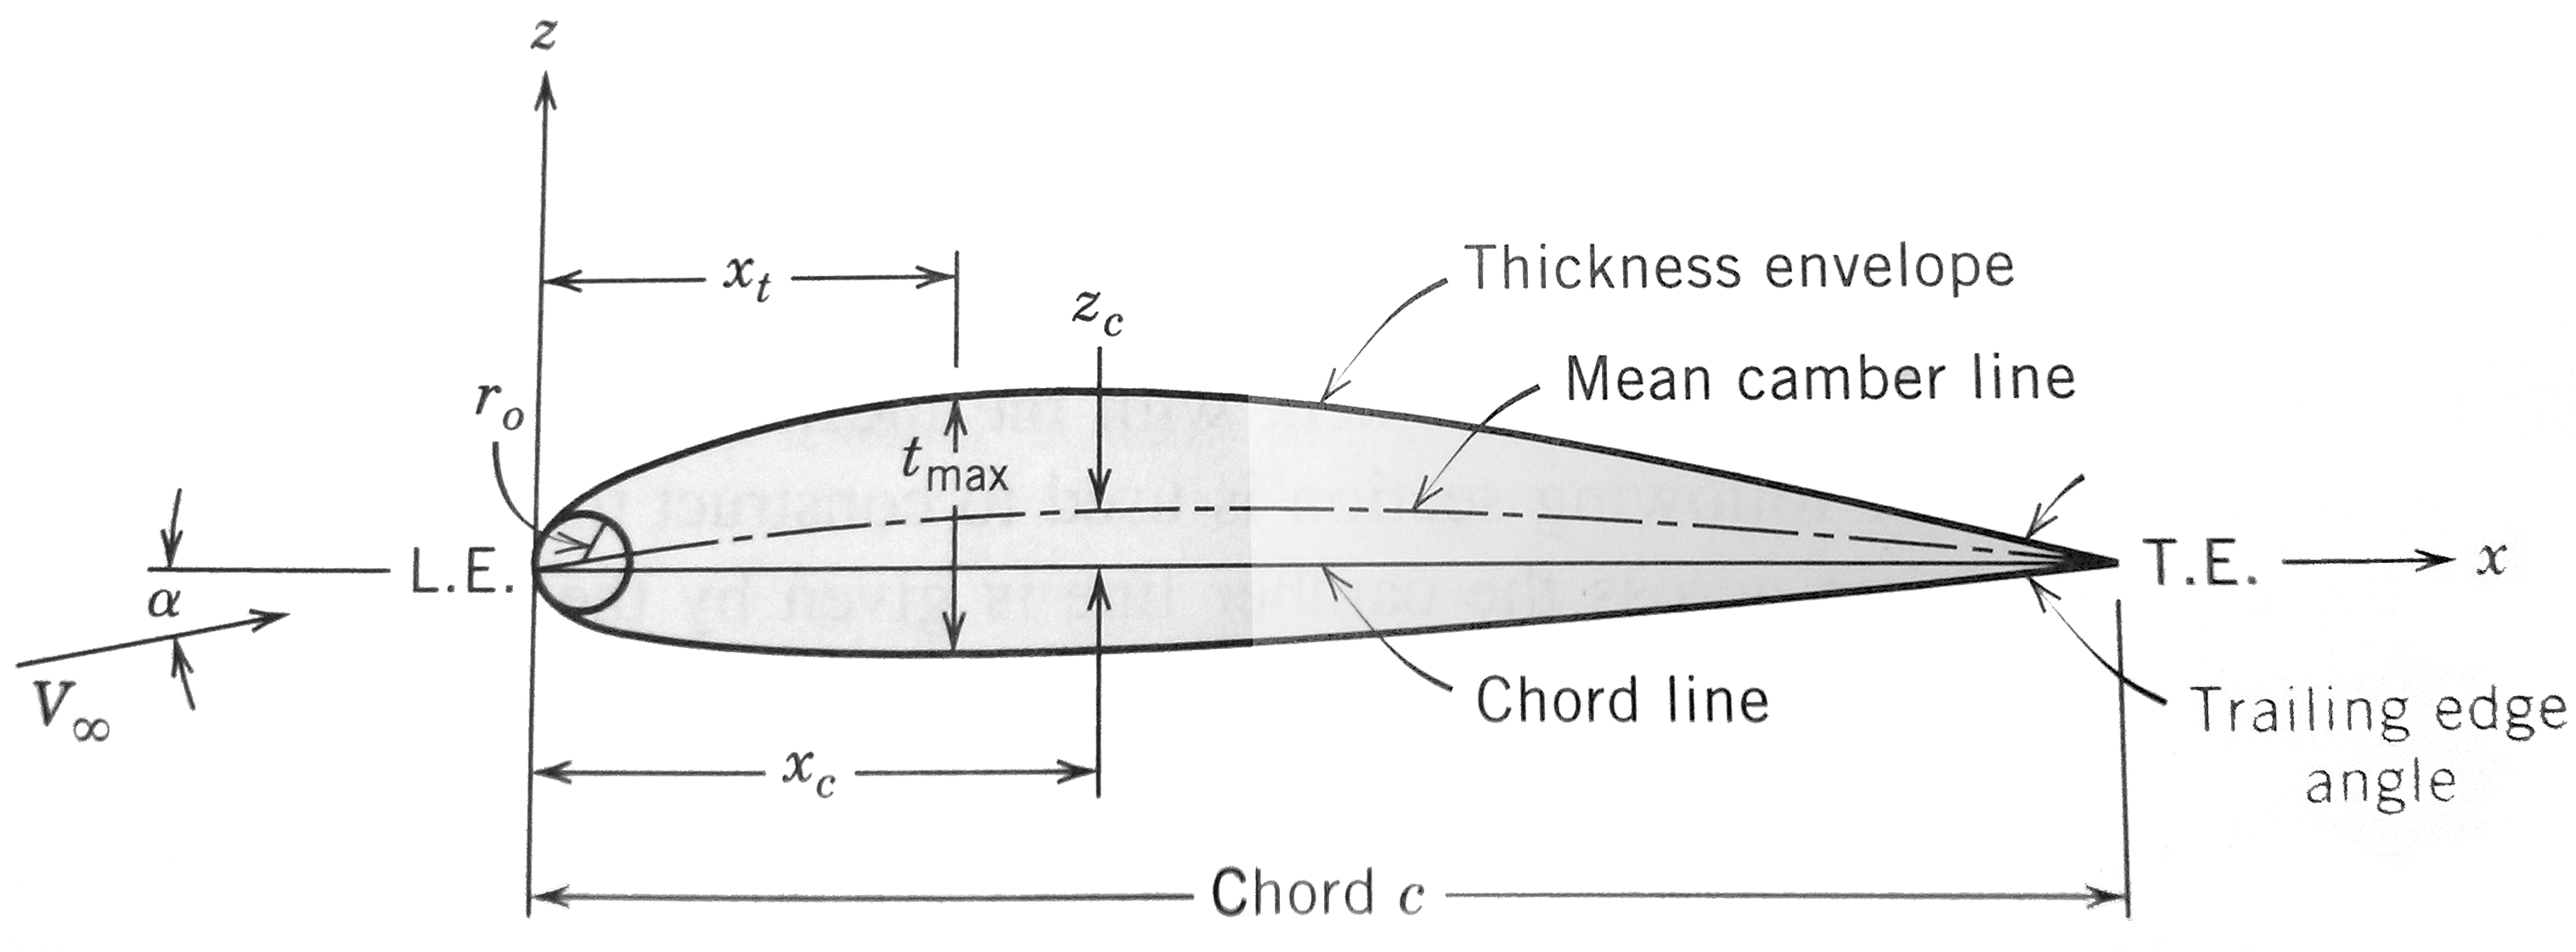
\includegraphics[width=\imagewidth]{images/background/airfoil.png}
    \caption{A depiction of the geometric properties of airfoil. The image was obtained from~\cite{kuethe1986foundations}.}
    \label{fig:airfoil-geometry}
\end{figure}

\section{Chapter summary}
In this chapter we gave a basic description of a mesh as a mathematical model. In addition we defined the concept of the mesh a data structure and how it is used in computation. Finally, we explained the significance of the airfoil in order to have a framing context for our running example.

\chapter{Related works}
We present a selection of prior works which touch upon the area of mesh structure, or are related to it in appealing ways.
% \section{Structure is beneficial}



% - How do quad meshes with subregions of structure come about
% - Are they seen often


\section{Structure detection and extraction}


Of all the works discussed in this chapter, \cite{tautges2004moab}~by Tautges is the most similar. The paper discusses the merits of structured meshes in great depth. It also defines the concept of disparate structured regions in a mesh, and discusses strategies for fusing them into a hierarchy of structures. A structure construction algorithm is also discussed very briefly.


% Fast Neighborhood Search on Polygonal Meshes
% http://www.inf.ethz.ch/personal/dpanozzo/papers/EGIT11-RocDeGPanPup.pdf
% Dude et al tackle the specific problem of neighborhood search by defining a spatial index, a hierarchy of clusters of vertices. Their method yields an approximation, ours is exact, with the mesh model left completely unaltered. However, we can learn a few things.

% The problem of indirections and its derivatives (non-contiguous memory access and its impact on cache hierarchy) is cited/highlighted as a key motivation in basing their mesh data structure on a geometric model, i.e. the spatial index. We undertake the opposite approach, viewing geometric data as mere associative data attached to a topological mesh model.

Adapting the mesh model to use a structured representation for the benefit of the relevant application domain is common practice.
Rocca et al.~\cite{rocca2011fast} address the particular problem of neighbourhood search: finding the set of vertices within a certain distance from a given vertex. They define a spatial index, a hierarchy of vertex clusters, that yields good approximations to neighbourhood search queries.

The problem of memory access indirections, associated with representing the mesh topology, is cited as a key motivation for basing their mesh data structure (the aforementioned spatial index) on a geometric model which does not require storing topological information. This is in sharp contrast to our approach of transforming the mesh topology representation, and treating the mesh geometry as arbitrary associated data.



% Motorcycle Graphs: Canonical Quad Mesh Partitioning
% http://www.ics.uci.edu/~goodrich/pubs/geomproc.pdf
% Whilst the motivations are different (mesh compression AND mesh isomorphism) the approach is similar:
% ``The simplest quadrilateral meshes are structured meshes, in which connections between quadrilaterals form a regular grid, but in complicated domains it may be necessary to use semi-regular meshes in which this structure is interrupted by a small number of extraordinary vertices that do not have degree four. We study how to partition a semi-regular mesh into a small number of structured submeshes.''


% ``To ensure that isomorphisms will always be found when they exist, our partition must be canonical: the same mesh must always generate the same partition. The partitioning algorithm we describe has this property.''
% We do not care about this property per se. There may be multiple optimal solutions for structure detection, for example.


% ``Additionally, these techniques may apply to areas beyond graphics such as scientific computation. Code for the finite element method can be greatly streamlined when applied to structured quadrilateral meshes. By partitioning unstructured meshes into structured submeshes, it should be possible to achieve similar speedups for semi-regular meshes.''

Eppstein et al.~\cite{eppstein2008motorcycle} describe a method for partitioning quadrilateral meshes into structured regions using the \emph{motorcycle graph} construction, whose inspiration came from the 1982 movie Tron. The algorithm works by placing particles on each \emph{extraordinary} vertex\footnote{\label{footnote:extraordinary-vertices} This is in contrast to an \emph{ordinary} vertex, which the authors define as ``a non-boundary vertex incident with four edges or a boundary vertex incident with at most three edges.''} in the mesh, and advancing them along edges until they collide. The enclosed regions formed by the paths represent structured regions.

Whilst the motivations are different, with the emphasis on applications in mesh compression and detecting mesh isomorphisms, the approach may be applicable to the scientific computation domain. Indeed, the authors state this explicitly:
\begin{quote}
These techniques may apply to areas beyond graphics such as scientific computation. Code for the finite element method can be greatly streamlined when applied to structured quadrilateral meshes. By partitioning unstructured meshes into structured sub-meshes, it should be possible to achieve similar speedups for semi-regular meshes.
\end{quote}

We note, however, that the method makes a stronger assumption about the mesh, in that its ``structure is interrupted by a \emph{small number} of extraordinary vertices that do not have degree four [emphasis added]''.


% There exist processes which explicitly attempt to produce semi-structured meshes, for example *BELOW* which uses domain specific knowledge about the source object to find long strips which can be made into quads.
% Automatic Decomposition and Efficient Semi-Structured Meshing of Complex Solids
% http://www.imr.sandia.gov/papers/imr20/Makem.pdf

Makem et al.~\cite{makem2012automatic} utilise properties of the modelled object to generate meshes with structured regions inherent. The presented method detects long thin shapes with simply defined geometry, such as length and curvature, and generates an appropriate structured region representing these shapes.



\section{Structure in parallel computation}
There is a plethora of work on mesh partitioning optimised for parallel computation. The techniques presented often frame their objectives around these maxims:
\begin{enumerate}
\item \label{item:maximize-locality} Maximize intra-partition locality, thereby minimizing cross-partition communication.
\item \label{item:minimize-size} Minimize partition size, subject to it being sufficiently large to counterbalance the communication overheads.
\item \label{item:maximize-number} The partitions should be balanced and plentiful in number, so as to utilise parallelism.
``A parallel computation is often only as efficient as the evenness with which its workload is distributed over the processors in a parallel machine.''
\end{enumerate}

Objective~\ref{item:maximize-locality} is certainly a desirable property for our structured regions, and is in fact precisely what we set forth to perform.
On the other hand, objectives~\ref{item:minimize-size} and \ref{item:maximize-number} are rather misaligned with our needs; indeed, a monolithic structured region spanning the entire mesh would represent the best case for us.

Thus some of the techniques which hold these conflicting\footnote{The objectives are in conflict in our context. These objectives are more suited for their parallel context, naturally} objectives may not be fully compatible, though they undoubtedly offer helpful inspiration.

With that said, extending our techniques towards parallel computation is an obvious future step, and such future works should likely re-evaluate their objectives in lieu of this.



% Guide to Partitioning Unstructured Meshes for Parallel Computing
% http://www.hector.ac.uk/cse/reports/unstructured_partitioning.pdf
% Very briefly describes several tools used for partitioning the mesh

A technical report by Ridley~\cite{ridley2010guide} briefly discusses methods for partitioning a mesh so as to maximize spatial data locality, in other words adjacent elements tend to have memory locations that are close. The partitioning is applied by recursively bisecting the mesh geometrically, such that geometrically close points tend to cluster together. The emphasis of the report is towards improving the performance of parallel computation, but the benefits of partitioning extend to serial processing as well.



% Hierarchical Partitioning Techniques for Structured Adaptive Mesh Refinement Applications
% http://www.s3lab.ece.ufl.edu/publication/jsuper.pdf
% Partitions mesh to exploit parallel computation whilst minimizing communication costs. This is done by \emph{exploiting} the hierarchical structure in a mesh. The approach focuses on partitioning for purposes of parallel computation, which involves a) minimizing communication costs; and b) maximizing locality within partitions. We focus solely on B.
% For **future works**, however, A would come into the picture as well, which would add an interesting dimension to the problem for further exploration.
% ``This scheme uses space filling curves (SFC), which are a class of locality preserving recursive mappings from n-dimensional to 1-dimensional space.''
% ALSO, note that this is *dynamic*. We can do that too in the future? :)

Li et al.~\cite{li2004hierarchical} follow a similar theme of parallel computation, although their methods deal with adaptive mesh refinement, where a mesh is dynamically refined in regions with a high calculation error. The refinement process induces a hierarchical structure, which the presented partitioning algorithms aim to exploit.



% Hierarchical hybrid grids: data structures and core algorithms for multigrid
% http://onlinelibrary.wiley.com/store/10.1002/nla.382/asset/382_ftp.pdf?v=1&t=hw5h84yv&s=bbe650e186f348823036d7426c24bd554ea00c1b

Bergen et al.~\cite{bergen2004hierarchical} employ structure-aware mesh refinement techniques, which construct a hierarchy of structured regions with each iterative refinement to the mesh. It is suggested that different element types, such as edges and faces, refined and stored separately, such that their distinct structuredness can be represented.

Since we use a simple structure representation, we make use of augmented structured regions, with different elements' structured region represented in a hierarchy.



% Stencils and Problem Partitionings: Their Influence on the Performance of Multiple Processor Systems
% http://ieeexplore.ieee.org/ielx5/12/35266/01676980.pdf?tp=&arnumber=1676980&isnumber=35266
% Partitioning a mesh based on its memory-access stencil. Again this is parallel oriented. Could be useful in defining the shape of the map access!

Reed et al.~\cite{reed1987stencils} focus on obtaining partitions best-suited to the \emph{stencil structure} associated with a particular computation, that is its neighbour-access pattern. They derive partition shapes for some common stencil structures, optimised to minimise inter-partition communication costs.

Tang et al.~\cite{tang2011pochoir} present a full-fledged \emph{Pochoir Stencil Compiler}. It specifies a domain-specific language that allows users to write a higher-level specification of a stencil computation embedded in C++ code. The compiler then automatically generates very efficient \emph{cache-oblivious}\footnote{The authors of~\cite{frigo1999cache} define a cache oblivious algorithm as that which ``[does not contain] parameters (set at either compile-time or runtime that can be tuned to optimize the cache complexity for the particular cache size and line length''} parallel loops that execute the stencil computation.

As discussed in subsection~\ref{subsec:given-kernel-function}, this is similar to our approach, where the structured regions are detected on the basis of relation-maps, such as cell-vertex or edge-cell maps.


% \url{https://www.cs.sfu.ca/~bgb2/personal/papers/nand11miccai.pdf}
% Bruv et al describe in [REF] the ``[construction of] curvature based features detectors to detect tube-like and sheet-like structures in DTI [diffusion tensor MRI]''. Differential equation-based methods are applied to characterize the ``'structured-ness'' of various components of the generated image, in terms of feature detection. Our focus is on detecting structuring in a precise manner, rather than a characteristic approach.

% FOR FUTURE WORKS: The differential equation approach may be an interesting tangent for future work, for instance applying it to geometric information to deduce areas of likely structure.


% \url{http://ieeexplore.ieee.org/ielx7/83/6490370/06476010.pdf?tp=&arnumber=6476010&isnumber=6490370}
% Again, approximate/heuristical image-based structure detection. The paper mentions low-level and high-level pattern detection.




% multiblock structured mesh partitioning algorithm
% http://www.geuz.org/pipermail/getdp/2000/000138.html
% Michael sends an email discussing stuff







% Structured Grid Computational Pattern
% (EITHER FROM:
%   Course: CS 4800, Fall 2010, School: Northeastern
%   OR
% Parallel Computing Laboratory - Berkley University)
% http://parlab.eecs.berkeley.edu/wiki/_media/patterns/structuredgrid-2.pdf
% http://view.eecs.berkeley.edu/wiki/Structured_Grids
% Good overview of the benefits of structured regions for computation.



\section{Exploiting structure}

% Approximate Topological Matching of Quadrilateral Meshes
% http://www.ics.uci.edu/~goodrich/pubs/approx-match.pdf
% Find matching subgraphs of two meshes, that is having the same topology.

% ``Our reason for using mesh compression instead is based on the desire to speed up the computation time in an algorithm that operates on quad meshes. Thus, our approach actually fits the spirit of other algorithms (e.g., see (33; 15; 14; 38)) that perform data compression so as to improve algorithmic performance.''
% Mentions reducing mesh representation for the purpose of improving computation time.


Eppstein et al.~\cite{eppstein2008approximate} explore the problem of approximate topological matching between given quadrilateral meshes, that is detecting isomorphisms between their submeshes. To this end they discuss various techniques based on \emph{particle shooting}\footnote{The motorcycle graph construction discussed in the paper by the same authors~\cite{eppstein2008motorcycle} is based on particle shooting.}: ``particles'' are placed on certain vertices (for example, extraordinary vertices\footref{footnote:extraordinary-vertices}) and are then ``'fired'' along the mesh using certain rules.

One such algorithm, termed ``The Greedy Algorithm'' by the authors, is shown to suffer from a problem when particles advancing along the same front can get out of sync. The problem is remarkably similar to our discussion about contiguous detection in subsection~\ref{subsec:contiguous-detection}.


% Opportunistic Data Structures with Applications
% http://people.unipmn.it/manzini/papers/focs00draft.pdf
% Discusses implicit data structures which minimize storage overheads due to auxiliary information


% \section{}


% Predictable memory access patterns versus *known* memory access pattern.



\section{Chapter summary}
In this chapter we discussed the similarities and differences between our work and that of a variety of published works centred at or homing around our scope of interest. We saw that the inefficiencies associated with unstructured representation are a common pain point, and we saw the great interest in the area of detecting structure to aid parallel computations. Some works presented exploited structure for other intriguing purposes.


\chapter{Rectangle growth strategy}
This chapter covers the detection of rectangular structured regions.

An abstract discussion of various properties of algorithms is presented, and the desirable traits brought forth by each.
Then, a selection of concrete algorithms are described, and their merits and weaknesses examined.


\section{Key concepts}
An \emph{absolute structured position} refers to the position of a structured element with respect to the boundaries of its structured region.
A \emph{relative structured position} refers to the position of a structured element with respect to other structured elements within its structured region. Figure~\ref{fig:structured-position} shows this through an example.


%% Relative vs absolute
\begin{figure}
\newcommand{\nodesize}{1.2}
\newcommand{\rows}{4}
\newcommand{\cols}{4}
\newcommand{\rowsize}{\rows*\nodesize}
\newcommand{\colsize}{\cols*\nodesize+2*0.1}

% Node at position r, c, label
\newcommand{\nodeat}[3]{
	\pgfmathsetmacro{\lerow}{ (\rows - #1) * \nodesize - (\nodesize / 2) - 0.1}
	\pgfmathsetmacro{\lecol}{ (#2 * \nodesize) + (\nodesize / 2) + 0.1}
	\node at (\lecol, \lerow) {#3}
}

\sidebyside
{
	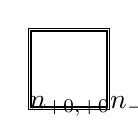
\begin{tikzpicture}
		\tikzstyle{every node}=[draw, shape=rectangle, minimum size=\nodesize cm, font=\small];
		\draw[double] (0,0) rectangle (\colsize,\rowsize);
		\nodeat{2}{1} {$n_{+0,+0}$};
		\nodeat{1}{1} {$n_{-1,+0}$};
		\nodeat{2}{2} {$n_{+0,+1}$};
	\end{tikzpicture}
	\caption{Relative structured position\label{fig:relative-structured-position}}
}
{
	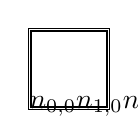
\begin{tikzpicture}
		\tikzstyle{every node}=[draw, shape=rectangle, minimum size=\nodesize cm, font=\small];
		\draw[double] (0,0) rectangle (\colsize,\rowsize);
		\nodeat{0}{0} {$n_{0,0}$};
		\nodeat{1}{0} {$n_{1,0}$};
		\nodeat{0}{1} {$n_{0,1}$};
	\end{tikzpicture}
	\caption{Absolute structured position\label{fig:absolute-structured-position}}
}
\caption{Depiction of \emph{relative} structured position versus \emph{absolute} structured position. The row and column counts are increasing down and to the right, respectively. The borders indicate structured regions, whose origin resides in the top-left corner.\label{fig:structured-position}}
\end{figure}



\section{Properties of detection algorithm}

\subsection{Eager detection}
An eager (or greedy) detection algorithm will include every structured element if finds immediately, regardless of the long term consequences. While this strategy may lead to suboptimal results, it avoids backtracking the structure detection which may be prohibitively costly. Figure~\ref{fig:eager-detection} depicts the sub-optimality of eager detection in contrast with non-eager detection.


\begin{figure}
\pgfplotstableread{
	2 2 2 2 2 2 0
	2 2 1 2 2 0 0
	0 0 1 0 0 0 0
	0 0 1 0 0 0 0
}{\eagermatrix}
\pgfplotstableread{
	2 2 2 2 2 2 0
	2 2 0 2 2 0 0
	1 1 1 1 1 1 1
	1 1 1 1 1 1 1
}{\noneagermatrix}

\sidebyside
{
	\drawmatrix[cell wd=0.6, cell ht=0.6]{\eagermatrix}
	\caption{Eager detection may greedily add the northern cell, yielding a suboptimal structured region.}
}
{
	\drawmatrix[cell wd=0.6, cell ht=0.6]{\noneagermatrix}
	\caption{A non-eager algorithm could instead decide to ignore the northern cell, yielding a larger structured region.}
}
\caption{Eager versus non-eager detection. Black cells and white cells denote unstructured and structured elements, respectively. Red cells denote structured elements detected as forming a rectangular structured region.\label{fig:eager-detection}}
\end{figure}



\subsection{Contiguous detection}
\label{subsec:contiguous-detection}
An algorithm which exhibits continuous detection always adds a structured element which is contiguous to the structured region thus far. The implication is that the relative structured position is always known. This greatly simplifies detection, as all adjacent structured elements are known at any point in time, and structured elements need not be repositioned in the structured region. Figure~\ref{fig:contiguous-detection} contrasts contiguous detection with non-contiguous detection.

In the case of non-contiguous detection, any non-contiguous blobs need to be consolidated. These blobs may be one of three cases:
\begin{enumerate}
\item Disjoint
These may simply be taken as two separate structured regions.

\item Compatible
The blobs can be merged in a lossless manner to form a single structured region.

\item Incompatible
The blobs cannot be merged without loss of structure due to inconsistencies between the blobs. It is then necessary to discard some structured elements.
\end{enumerate}

Examples of the three cases are shown in figure~\ref{fig:non-contiguous-detection}.


% Contiguous versus non-contiguous
\begin{figure}
\pgfplotstableread{
	0 1 1 1 0 0 0 0 0
	0 1 1 1 1 0 0 0 0
	0 1 1 1 0 0 0 0 0
	0 0 1 0 0 0 0 0 0
	0 0 0 0 0 0 0 0 0
}{\contiguousmatrix}
\pgfplotstableread{
	0 1 1 1 0 0 0 0 0
	0 1 1 1 1 0 0 1 0
	0 1 1 1 0 0 1 1 0
	0 0 1 0 0 0 0 0 0
	0 0 0 0 0 0 0 0 0
}{\noncontiguousmatrix}

\sidebyside
{
	\drawmatrix[cell wd=0.6, cell ht=0.6]{\contiguousmatrix}
	\caption{Contiguous detection always adds cells adjacent to the structured region detected thus far.}
}
{
	\drawmatrix[cell wd=0.6, cell ht=0.6]{\noncontiguousmatrix}
	\caption{Non-contiguous detection may add cells which do not border the structured region detected thus far.}
}
\caption{Contiguous detection versus non-contiguous detection algorithms. White cells denote structured elements which have not been added to the structured region. Red cells denote structured elements detected thus far.\label{fig:contiguous-detection}}
\end{figure}

% Types of non-contiguous
\begin{figure}
\sidebysidethreevertical
{
	\includesvg[svgpath=images/detection-algorithms/,width=60mm]{disjoint-blobs}
	\caption{Disjoint blobs of structured elements.}
}
{
	\includesvg[svgpath=images/detection-algorithms/,width=60mm]{compatible-blobs}
	\caption{Compatible blobs of structured elements.}
}
{
	\includesvg[svgpath=images/detection-algorithms/,width=60mm]{incompatible-blobs}
	\caption{Incompatible blobs of structured elements. The two dashed cells are not adjacent in the mesh, but if added as structured element they would have adjacent positions in the structured region.}
}
\caption{Cases that may arise with non-contiguous detection.\label{fig:non-contiguous-detection}}
\end{figure}


\subsection{Post processing requirements}
Different algorithms will require different levels of post-processing in order to yield a rectangular structured region. Some may require a simple operation, such as trimming incomplete rows, while others may require more complex operations to achieve this goal.


\subsection{Detection traversal patterns}
The order in which structured elements are detected in a structured region is important; it imposes some constraints on the data structure representing it. Given the dimensions of the structured region, and knowledge of the absolute structured positions of elements as they are discovered, a simple 2D array allocation would suffice. Any detection order, as is convenient, may be used in this case. However, neither of those facts are known a priori in general.

Various detection traversals orders and their merits are discussed below. Figure~\ref{fig:detection-traversal-patterns} outlines some examples.

\subsubsection{Single-row append-only}
\label{append-detection}
The structured region is grown in a constant direction, for example a single row of structured elements, appended to consecutively. This can be implemented efficiently using either a singly-linked list or a dynamic array with amortized constant time append operation.

\subsubsection{Single-row append/prepend}
\label{append-prepend-detection}
The structured region is grown in either of two directions, for example a single row of structured elements, appended and prepended to. This can be implemented efficiently using a double-ended queue with amortized constant time append and prepend operations.

\subsubsection{Row-oriented detection}
The structured region is represented as a group of rows, with the elements in individual rows grown using one of the above methods. The order in which the rows themselves are grown may also be utilize the same methods, with a nested data structure being a suitable implementation. For example, if rows are detected in an append-only fashion, and the individual elements are detected using append and prepend operations, then a suitable data structure would be a singly-linked list of double-ended queues.

\subsubsection{Indeterminate order detection}
The structured region is grown in a non-linear order: grown elements may not always be contiguous to the structured region thus far. If the growth is indeed non-contiguous, the relative structured positions are \emph{not} always known, and structured elements may need to be repositioned. A possible implementation would be a jagged 2D array, that is an array of arrays, which is expanded as needed. A flat-array-based 2D array would (in the worst case) require reallocating all elements upon expansion, as opposed to reallocating a single row in the case of a jagged 2D array.


% Detection traversal patterns
\begin{figure}
\sidebysidefour
{
	\includesvg[svgpath=images/detection-algorithms/,height=10mm]{append-detection}
	\caption{Single-row append detection.}
}
{
	\includesvg[svgpath=images/detection-algorithms/,height=10mm]{append-prepend-detection}
	\caption{Single-row append/prepend detection.}
}
{
	\includesvg[svgpath=images/detection-algorithms/,height=34mm]{row-oriented}
	\caption{Row-oriented detection, with rows detected in an append-only fashion, and elements within rows in an append/prepend fashion.}
}
{
	\includesvg[svgpath=images/detection-algorithms/,height=51mm]{indeterminate-detection}
	\caption{Indeterminate order detection. Note that some possible regions of expansions are not adjacent to the presently detected structured region.}
}
\caption{Examples of detection traversal patterns. The red blocks represent presently detected structured regions. The dashed pink blocks represent possible regions for expansion.\label{fig:detection-traversal-patterns}}
\end{figure}




Consider contiguity in a figure!!!!

---------------------
                    |
                    |
          A         |
        -------------
     B  | C |
        |----
        |
---------

If the the region were to be grown to include include element C, it must be the case that C is adjacent to both A and B, but is not adjacent to any other structured element thus far. Since the structure is always contiguous, we know at every point whether any two structured elements ought to be adjacent.


\section{Detection algorithms}

\subsection{Length-first search}

\begin{enumerate}
\item Starting from a seed vertex, grow a quad.

\item The quad is grown along one axis, both forwards and backwards, as far as possible, forming the length of the structured region. This is a per-row append/prepend traversal.
\item The row grown above is extended along the orthogonal axis, both forwards and backwards, as far as possible. Each expanded row must have the length of the initial row exactly, forming the width of the structure region. This is a row-oriented append/prepend traversal.
\end{enumerate}

The detection is clearly contiguous, with all structured element insertions running in amortized constant time. Only a constant amount of extra storage is required.

The algorithm is also an eager one, deciding the length of the structured region based on the first row it detects. This simple approach, however, can result in suboptimal detection.



\subsection{Descending-staircase search}
\begin{enumerate}
\item Follow the same steps as in length-first search, with one exception: in step~\ref{step:row-expansion}, each expanded row may have a length which is at most the length of its predecessor.
\item Find the rectangle with the maximum area, using an algorithm such as XXXXXX.
\end{enumerate}



Two types of techniques exist: seed-based, and global based. A seed-based technique starts with a seed, and grows from there. A global-based technique starts with all the orthogonal axis

\chapter{Structure Extraction}
\label{chap:detect-quad-grid}
Taking forth our length-first search algorithm, we expand fill in the details glossed over by our earlier discussion, delineating it into a formal algorithmic specification.

% Initial vertex
\newcommand{\vinit}{v_{init}}

\newcommand{\Quad}[4]{\begin{bmatrix} #1 & #2 \\ #3 & #4 \end{bmatrix}}

% Initial quad
\newcommand{\Qinit}{\Quad{n_{1,1}} {n_{1,2}} {n_{2,1}} {n_{2,2}} }

% Initial quad mirrored about y-axis
\newcommand{\Qinitmirror}{\Quad {n_{1,2}} {n_{1,1}} {n_{2,2}} {n_{2,1}}}



\section{Inputs}
\begin{enumerate}
\item A non-reflexive and symmetric vertex-vertex adjacency relation:
$$ \AdjVV: \VertexSet \mapsto \powerset{\VertexSet} $$

\item A set of visited vertices
$$ \Visited \subseteq \VertexSet $$

\item An unvisited start vertex
$$ \vinit \in \VertexSet \setminus \Visited $$
\end{enumerate}


\section{Outputs}
\begin{enumerate}
\item A structured set of vertices $\Structured \subseteq \VertexSet \setminus \Visited $ forming the extracted structured region.
The vertices $\Structured$ are structured on a 2-dimensional Cartesian lattice with $m$ rows and $n$ columns.
\end{enumerate}


%%%% PHASE 1

%% Phase 1 summary
\section{Phase 1: Grow a quad}
\label{sec:grow_a_quad}
Starting from the initial vertex $\vinit$, call it $n_{1,1}$, we would like to discover three other vertices $n_{1,2}$, $n_{2,1}$, and $n_{2,2}$ such that $\Qinit$ forms a valid quad in a structured quad region. They must satisfy the following constraints:

\begin{itemize}
\item Each of the four vertices must have exactly 4 neighbours.
\item Each of the following pairs of vertices are neighbours: $n_{1,1}$~and~$n_{1,2}$ ; $n_{1,2}$~and~$n_{2,2}$ ; $n_{2,2}$~and~$n_{2,1}$ ; $n_{2,1}$~and~$n_{1,1}$.
\item Each of the vertices must \emph{not} neighbour any vertex that has been visited thus far, apart from those vertices explicitly mentioned.
\end{itemize}

%% Phase 1 diagram

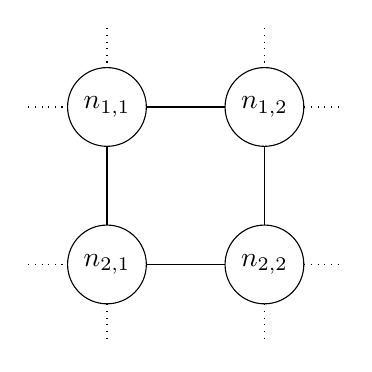
\begin{tikzpicture}[scale=1]
	% Default action for each node
	\tikzstyle{every node}=[draw, shape=circle, minimum size=1cm];

										\coordinate (northleft) at (0, 2);	\coordinate (northright) at (2, 2);
	\coordinate (westup) at (-1,1);		\node (r1c1) at (0,1) {$n_{1,1}$};	\node (r1c2) at (2,1) {$n_{1,2}$};	\coordinate (eastup) at (3,1);
	\coordinate (westdown) at (-1,-1);	\node (r2c1) at (0,-1) {$n_{2,1}$};	\node (r2c2) at (2,-1) {$n_{2,2}$};	\coordinate (eastdown) at (3,-1);
										\coordinate (southleft) at (0, -2);	\coordinate (southright) at (2, -2);

	% Horizontals
	\draw[outside] (westup) -- (r1c1);
	\draw (r1c1) -- (r1c2);
	\draw[outside] (r1c2) -- (eastup);

	\draw[outside] (westdown) -- (r2c1);
	\draw (r2c1) -- (r2c2);
	\draw[outside] (r2c2) -- (eastdown);

	% Verticals
	\draw[outside] (northleft) -- (r1c1);
	\draw (r1c1) -- (r2c1);
	\draw[outside] (r2c1) -- (southleft);

	\draw[outside] (northright) -- (r1c2);
	\draw (r1c2) -- (r2c2);
	\draw[outside] (r2c2) -- (southright);
\end{tikzpicture}

%% Phase 1 algorithm

\subsection{Algorithm}

\begin{enumerate}
\item If $\vinit$ does not have exactly 4 neighbours, that is $ \card{\AdjVV(\vinit)} \neq 4 $, return immediately with $\Structured = \varnothing$.
\item Let $ n_{1,1} = \vinit $, and let $ a, b, c \in \AdjVV(\vinit) $ be distinct vertex neighbours of $\vinit$. Consider vertices $a$ and $b$. If they do not both have exactly 4 neighbours, then they cannot form a part of a structured quad region. Return immediately with $\Structured = \varnothing$.

\item Otherwise, there are three cases:

	%%%% BEGIN THREE CASES
	\begin{enumerate}

	%% Straight line case
	\item $a$ and $b$ have exactly one neighbour in common, which must be $n_{1,1}$ by construction, expressed by:
	$$ \card{\AdjVV(a) \cap \AdjVV(b)} = 1$$
	$a, n_{1,1}, b $ are \emph{topologically} along a straight line of a structured grid, and hence cannot form a quad.
	We therefore consider $b$, $n_{1,1}$, and  $c$ instead as candidates, letting $n_{2,1} = b$ and $n_{1,2} = c$.
	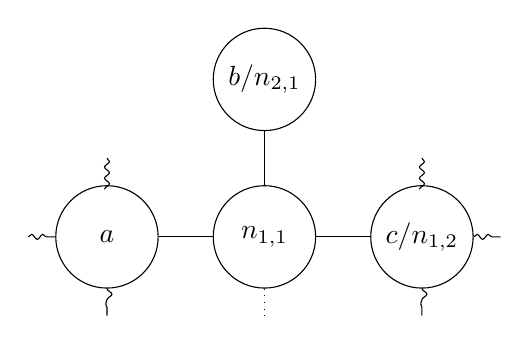
\begin{tikzpicture}
		% Default action for each node
		\tikzstyle{every node}=[draw, shape=circle, minimum size=1.3cm];

										\coordinate (northleft) at (-1,2);	\node (b) at (1,3) {$b / n_{2,1}$};	\coordinate (northright) at (3,2);
		\coordinate (west) at (-2,1);	\node (a) at (-1,1) {$a$};			\node (n11) at (1,1) {$n_{1,1}$};	\node (c) at (3,1) {$c / n_{1,2}$};	\coordinate (east) at (4,1);
										\coordinate (southleft) at (-1,0);	\coordinate (southmid) at (1,0);	\coordinate (southright) at (3,0);

		% Horizontals
		\draw[anywhere] (west) -- (a);
		\draw (a) -- (n11) -- (c);
		\draw[anywhere] (c) -- (east);

		% Verticals
		\draw[anywhere] (northleft) -- (a) -- (southleft);
		\draw (b) -- (n11);
		\draw[outside] (n11) -- (southmid);
		\draw[anywhere] (northright) -- (c) -- (southright);
	\end{tikzpicture}


	%% Angle case
	\item $a$ and $b$ have exactly two neighbours in common, one of which must be $n_{1,1}$ by construction, expressed by:
	$$ \card{\AdjVV(a) \cap \AdjVV(b)} = 2$$
	We continue with vertices $a$, $n_{1,1}$, and $b$ as candidates, letting $n_{2,1} = a$ and $n_{1,2} = b$.
	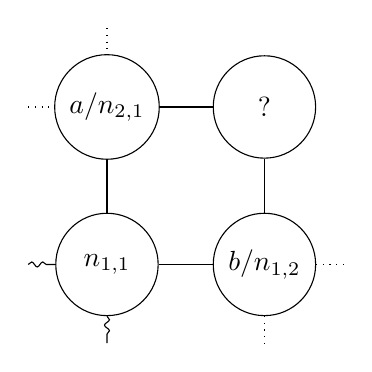
\begin{tikzpicture}
		% Default action for each node
		\tikzstyle{every node}=[draw, shape=circle, minimum size=1.3cm];

											\coordinate (northleft) at (-1,4);		\coordinate (northright) at (1,4);
		\coordinate (westup) at (-2,3);		\node (a) at (-1,3) {$a / n_{2,1}$};	\node (d) at (1,3) {$?$};			\coordinate (eastup) at (2,3);
		\coordinate (westdown) at (-2,1);	\node (n11) at (-1,1) {$n_{1,1}$};		\node (b) at (1,1) {$b / n_{1,2}$};	\coordinate (eastdown) at (2,1);
											\coordinate (southleft) at (-1,0);		\coordinate (southright) at (1,0);



		\draw[outside] (westup) -- (a);
		\draw (a) -- (d);
		% \draw (d) -- (eastup);

		\draw[anywhere] (westdown) -- (n11);
		\draw (n11) -- (b);
		\draw[outside] (b) -- (eastdown);

		\draw[outside] (northleft) -- (a);
		\draw (a) -- (n11);
		\draw[anywhere] (n11) -- (southleft);

		% \draw (northright) -- (d);
		\draw (d) -- (b);
		\draw[outside] (b) -- (southright);

	\end{tikzpicture}


	\item $a$ and $b$ have more than two neighbours in common\footnote{Note that the set is non-empty by construction}, expressed by:
	$$ \card{\AdjVV(a) \cap \AdjVV(b)} > 2$$
	We cannot form a quad, and hence return immediately with $\Structured = \varnothing$.

	\end{enumerate}
	%%%% END THREE CASES

\item Find the common neighbours of $n_{2,1}$ and $n_{1,2}$. If these are not exactly two neighbours, return immediately with $\Structured = \varnothing$.

\item One of the two neighbours must be $n_{1,1}$ by construction. Let the other neighbour be $n_{2,2}$.

\item Let $N = \{ n_{1,1}, n_{1,2}, n_{2,1}, n_{2,2} \}$. If any vertex $n \in N$ is in $\Visited$, that is $N \cap \Visited \neq \varnothing$, then return immediately with $\Structured = \varnothing$. Otherwise add the vertices in $N$ to $\Visited$.

\item Ensure for every vertex $n \in N$ that its visited neighbours, $\AdjVV(n) \cap \Visited$, are exactly those explicitly stated above. If this is not the case, remove $N$ from $\Visited$ and return immediately with $\Structured = \varnothing$.


\item Set $\Structured = \Qinit$, and continue to the next phase.

The structured region looks as follows thus far.
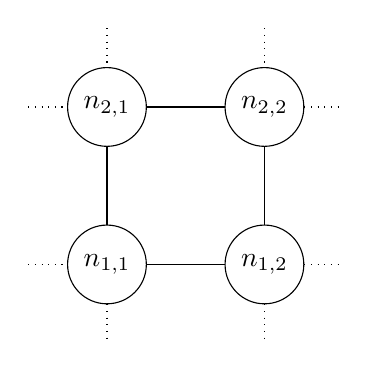
\begin{tikzpicture}
	% Default action for each node
	\tikzstyle{every node}=[draw, shape=circle, minimum size=1cm];

										\coordinate (northleft) at (-1,4);	\coordinate (northright) at (1,4);
	\coordinate (westup) at (-2,3);		\node (n21) at (-1,3) {$n_{2,1}$};	\node (n22) at (1,3) {$n_{2,2}$};	\coordinate (eastup) at (2,3);
	\coordinate (westdown) at (-2,1);	\node (n11) at (-1,1) {$n_{1,1}$};	\node (n12) at (1,1) {$n_{1,2}$};	\coordinate (eastdown) at (2,1);
										\coordinate (southleft) at (-1,0);	\coordinate (southright) at (1,0);

	\draw[outside] (westup) -- (n21);
	\draw (n21) -- (n22);
	\draw[outside] (n22) -- (eastup);

	\draw[outside] (westdown) -- (n11);
	\draw (n11) -- (n12);
	\draw[outside] (n12) -- (eastdown);

	\draw[outside] (northleft) -- (n21);
	\draw (n21) -- (n11);
	\draw[outside] (n11) -- (southleft);

	\draw[outside] (northright) -- (n22);
	\draw (n22) -- (n12);
	\draw[outside] (n12) -- (southright);

\end{tikzpicture}

\end{enumerate}








%%%% Definition A

%% Definition A summary
\section{Function definition: Extend a quad (used in phase 2)}
Starting from $Q_i = \Quad {n_{1,i}} {n_{1,i+1}} {n_{2,i}} {n_{2,i+1}}$, which must be a valid quad in a structured region, we would like to find two more vertices $n_{1, i+2}$ and $n_{2,i+2}$, such that $Q_{i+1} = \Quad {n_{1,i+1}} {n_{1,i+2}} {n_{2,i+1}} {n_{2,i+2}}$ forms a valid quad in a structured quad region. They must satisfy the following constraints:

\begin{itemize}
\item Each of the vertices $n_{1, i+2}$ and $n_{2,i+2}$ must have exactly 4 neighbours.
\item Each of the following pairs of vertices are neighbours: $n_{1,i+1}$~and~$n_{1,i+2}$ ; $n_{2,i+1}$~and~$n_{2,i+2}$ ; $n_{1,i+2}$~and~$n_{2,i+2}$.
\item Each of the vertices $n_{1, i+2}$ and $n_{2,i+2}$ must \emph{not} neighbour any vertex that has been visited thus far, apart from those vertices explicitly mentioned.
\end{itemize}

%% Definition A diagram

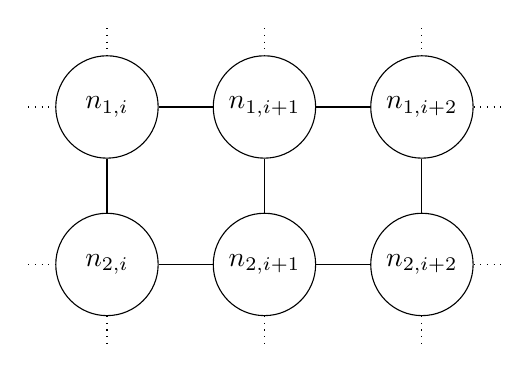
\begin{tikzpicture}[scale=1]
	% Default action for each node
	\tikzstyle{every node}=[draw, shape=circle, minimum size=1.3cm];

										\coordinate (northleft) at (0, 2);	\coordinate (northmid) at (2, 2);		\coordinate (northright) at (4, 2);
	\coordinate (westup) at (-1,1);		\node (r1c1) at (0,1) {$n_{1,i}$};	\node (r1c2) at (2,1) {$n_{1,i+1}$};	\node (r1c3) at (4,1) {$n_{1,i+2}$};	\coordinate (eastup) at (5,1);
	\coordinate (westdown) at (-1,-1);	\node (r2c1) at (0,-1) {$n_{2,i}$};	\node (r2c2) at (2,-1) {$n_{2,i+1}$};	\node (r2c3) at (4,-1) {$n_{2,i+2}$};	\coordinate (eastdown) at (5,-1);
										\coordinate (southleft) at (0, -2);	\coordinate (southmid) at (2, -2);		\coordinate (southright) at (4, -2);

	% Horizontals
	\draw[outside] (westup) -- (r1c1);
	\draw (r1c1) -- (r1c2);
	\draw (r1c2) -- (r1c3);
	\draw[outside] (r1c3) -- (eastup);

	\draw[outside] (westdown) -- (r2c1);
	\draw (r2c1) -- (r2c2);
	\draw (r2c2) -- (r2c3);
	\draw[outside] (r2c3) -- (eastdown);

	% Verticals
	\draw[outside] (northleft) -- (r1c1);
	\draw (r1c1) -- (r2c1);
	\draw[outside] (r2c1) -- (southleft);

	\draw[outside] (northmid) -- (r1c2);
	\draw (r1c2) -- (r2c2);
	\draw[outside] (r2c2) -- (southmid);

	\draw[outside] (northright) -- (r1c3);
	\draw (r1c3) -- (r2c3);
	\draw[outside] (r2c3) -- (southright);
\end{tikzpicture}


%% Definition A algorithm

\subsection{Algorithm}

\begin{enumerate}
\item $n_{1,i+1}$ has 4 neighbours, which include $n_{1,i}$ and $n_{2,i+1}$. Call the remaining 2 neighbours $a$ and $b$. This is expressed by:
$$ \AdjVV(n_{1,i+1}) \setminus \{ n_{1,i} , n_{2,i+1} \} = \{ a , b \} $$

\item $n_{2,i+1}$ has 4 neighbours, which include $n_{2,i}$ and $n_{1,i+1}$. Call the remaining 2 neighbours $c$ and $d$.
$$ \AdjVV(n_{2,i+1}) \setminus \{ n_{2,i} , n_{1,i+1} \} = \{ c , d \} $$

\item Choose two vertices $n_{1,i+2} \in \{ a , b \}$ and $n_{2,i+2} \in \{ c , d \}$ such that $n_{1,i+2}$ and $n_{2,i+2}$ are neighbours, which is expressible\footnote{Or equivalently (by symmetry of $\AdjVV$) $n_{2,i+2} \in \AdjVV(n_{1,i+2})$} as:
$$n_{1,i+2} \in \AdjVV(n_{2,i+2})$$
and such that they each have exactly 4 neighbours. If no such vertices $n_{1,i+2}$ and $n_{2,i+2}$ exist, fail the procedure.


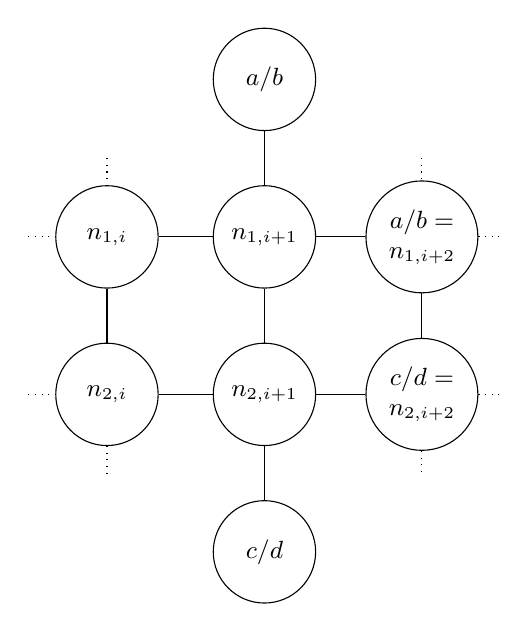
\begin{tikzpicture}[scale=1]
	% Default action for each node
	\tikzstyle{every node}=[draw, shape=circle, minimum size=1.3cm, align=center, font=\small];

										\coordinate (northleft) at (0, 2);	\coordinate (northmid) at (2, 2);		\coordinate (northright) at (4, 2);
	\coordinate (westup) at (-1,3);											\node (abup) at (2,3) {$a/b$};			\coordinate (eastup) at (5,1);
	\coordinate (westmid) at (-1,1);	\node (r1c1) at (0,1) {$n_{1,i}$};	\node (r1c2) at (2,1) {$n_{1,i+1}$};	\node (r1c3) at (4,1) {$a/b =$ \\ $n_{1,i+2}$};		\coordinate (eastmid) at (5,1);
	\coordinate (westdown) at (-1,-1);	\node (r2c1) at (0,-1) {$n_{2,i}$};	\node (r2c2) at (2,-1) {$n_{2,i+1}$};	\node (r2c3) at (4,-1) {$c/d =$ \\ $n_{2,i+2}$};	\coordinate (eastdown) at (5,-1);
	\coordinate (westlow) at (-1,-3);										\node (cdup) at (2,-3) {$c/d$};			\coordinate (eastlow) at (5,1);
										\coordinate (southleft) at (0, -2);	\coordinate (southmid) at (2, -2);		\coordinate (southright) at (4, -2);

	% Horizontals
	\draw[outside] (westmid) -- (r1c1);
	\draw (r1c1) -- (r1c2);
	\draw (r1c2) -- (r1c3);
	\draw[outside] (r1c3) -- (eastmid);

	\draw[outside] (westdown) -- (r2c1);
	\draw (r2c1) -- (r2c2);
	\draw (r2c2) -- (r2c3);
	\draw[outside] (r2c3) -- (eastdown);

	% Verticals
	\draw[outside] (northleft) -- (r1c1);
	\draw (r1c1) -- (r2c1);
	\draw[outside] (r2c1) -- (southleft);

	\draw (abup) -- (r1c2);
	\draw (r1c2) -- (r2c2);
	\draw (r2c2) -- (cdup);

	\draw[outside] (northright) -- (r1c3);
	\draw (r1c3) -- (r2c3);
	\draw[outside] (r2c3) -- (southright);
\end{tikzpicture}


\item If any of the two vertices $n_{1,i+2}$ and $n_{2,i+2}$ exists in $\Visited$, that is $\{ n_{1,i+2} , n_{2,i+2} \} \cap \Visited \neq \varnothing$, fail the procedure.
Otherwise add the two vertices to $\Visited$.

\item Ensure for every vertex $n \in \{ n_{1,i+2} , n_{2,i+2} \}$ that its visited neighbours, $\AdjVV(n) \cap \Visited$, are exactly those explicitly stated above. If this is not the case, remove $\{ n_{1,i+2} , n_{2,i+2} \}$ from $\Visited$ and fail the procedure.

\item Return the two vertices $n_{1,i+2}$ and $n_{2,i+2}$.
\end{enumerate}







%%%% PHASE 2

\section{Phase 2: Extend a row}
%% Phase 2.1 summary
``Extend a quad'' is iteratively applied, starting from $Q_1 = \Qinit$, to yield successive quads until it fails.
The resulting vertices are appended to the \emph{right} of $\Structured$ to form a single quad row in a structured quad region, or equivalently a successive pair of node rows.

%% Phase 2.1 diagram
\begin{tikzpicture}[scale=1]
	% Default action for each node
	\tikzstyle{every node}=[draw, shape=circle, minimum size=1.3cm];

	% MIDDLE

										\coordinate (northleft) at (0, 2);	\coordinate (northright) at (2, 2);
	\coordinate (westup) at (-1,1);		\node (r1c1) at (0,1) {$n_{1,1}$};	\node (r1c2) at (2,1) {$n_{1,2}$};		\coordinate (eastup) at (3,1);
	\coordinate (westdown) at (-1,-1);	\node (r2c1) at (0,-1) {$n_{2,1}$};	\node (r2c2) at (2,-1) {$n_{2,2}$};		\coordinate (eastdown) at (3,-1);
										\coordinate (southleft) at (0, -2);	\coordinate (southright) at (2, -2);

	% ellipses
	\coordinate (ellipsis westup) at (4,1);		\coordinate (ellipsis eastup) at (4.5,1);
	\coordinate (ellipsis westdown) at (4,-1);	\coordinate (ellipsis eastdown) at (4.5,-1);


	% RHS
											\coordinate (rhs north) at (6, 2);
	\coordinate (rhs westup) at (5,1);		\node (r1cn) at (6,1) {$n_{1,c_+}$};	\coordinate (rhs eastup) at (7,1);
	\coordinate (rhs westdown) at (5,-1);	\node (r2cn) at (6,-1) {$n_{2,c_+}$};	\coordinate (rhs eastdown) at (7,-1);
											\coordinate (rhs south) at (6, -2);



	% Horizontals
	\draw[outside] (westup) -- (r1c1);
	\draw (r1c1) -- (r1c2);
	\draw (r1c2) -- (r1c3);
	\draw (r1c3) -- (eastup);

	\draw[outside] (westdown) -- (r2c1);
	\draw (r2c1) -- (r2c2);
	\draw (r2c2) -- (r2c3);
	\draw (r2c3) -- (eastdown);

	\draw[ellipsis] (ellipsis westup) -- (ellipsis eastup);
	\draw[ellipsis] (ellipsis westdown) -- (ellipsis eastdown);


	\draw (rhs westup) -- (r1cn);
	\draw[outside] (r1cn) -- (rhs eastup);

	\draw (rhs westdown) -- (r2cn);
	\draw[outside] (r2cn) -- (rhs eastdown);

	% Verticals
	\draw[outside] (northleft) -- (r1c1);
	\draw (r1c1) -- (r2c1);
	\draw[outside] (r2c1) -- (southleft);

	\draw[outside] (northright) -- (r1c2);
	\draw (r1c2) -- (r2c2);
	\draw[outside] (r2c2) -- (southright);

	\draw[outside] (rhs north) -- (r1cn);
	\draw (r1cn) -- (r2cn);
	\draw[outside] (r2cn) -- (rhs south);
\end{tikzpicture}



%% Phase 2.2 summary
Next, ``Extend a quad'' is again iteratively applied, this time with $Q_1 = \Qinitmirror$, the mirror image of $Q_{init}$ about the y-axis.
The repeated application yields successive quads until the procedure fails.
The resulting vertices are appended to the \emph{left} of $\Structured$ to extend the existing quad row, or equivalently a successive pair of node rows.


%% Phase 2.2 diagram
\begin{tikzpicture}[scale=1]
	% Default action for each node
	\tikzstyle{every node}=[draw, shape=circle, minimum size=1.3cm];

	% LHS
												\coordinate (lhs north) at (-3.5, 2);
	\coordinate (lhs westup) at (-4.5,1);		\node (r1cm) at (-3.5,1) {$n_{1,c_{\!^{\_}}}$};		\coordinate (lhs eastup) at (-2.5,1);
	\coordinate (lhs westdown) at (-4.5,-1);	\node (r2cm) at (-3.5,-1) {$n_{2,c_{\!^{\_}}}$};	\coordinate (lhs eastdown) at (-2.5,-1);
												\coordinate (lhs south) at (-3.5, -2);

	% lhs ellipses
	\coordinate (lhs ellipsis westup) at (-2,1);	\coordinate (lhs ellipsis eastup) at (-1.5,1);
	\coordinate (lhs ellipsis westdown) at (-2,-1);	\coordinate (lhs ellipsis eastdown) at (-1.5,-1);


	% MIDDLE
										\coordinate (northleft) at (0, 2);	\coordinate (northright) at (2, 2);
	\coordinate (westup) at (-1,1);		\node (r1c1) at (0,1) {$n_{1,1}$};	\node (r1c2) at (2,1) {$n_{1,2}$};		\coordinate (eastup) at (3,1);
	\coordinate (westdown) at (-1,-1);	\node (r2c1) at (0,-1) {$n_{2,1}$};	\node (r2c2) at (2,-1) {$n_{2,2}$};		\coordinate (eastdown) at (3,-1);
										\coordinate (southleft) at (0, -2);	\coordinate (southright) at (2, -2);

	% rhs ellipses
	\coordinate (rhs ellipsis westup) at (4,1);		\coordinate (rhs ellipsis eastup) at (4.5,1);
	\coordinate (rhs ellipsis westdown) at (4,-1);	\coordinate (rhs ellipsis eastdown) at (4.5,-1);


	% RHS
											\coordinate (rhs north) at (6, 2);
	\coordinate (rhs westup) at (5,1);		\node (r1cn) at (6,1) {$n_{1,c_+}$};	\coordinate (rhs eastup) at (7,1);
	\coordinate (rhs westdown) at (5,-1);	\node (r2cn) at (6,-1) {$n_{2,c_+}$};	\coordinate (rhs eastdown) at (7,-1);
											\coordinate (rhs south) at (6, -2);



	% Horizontals
	\draw (westup) -- (r1c1);
	\draw (r1c1) -- (r1c2);
	\draw (r1c2) -- (r1c3);
	\draw (r1c3) -- (eastup);

	\draw(westdown) -- (r2c1);
	\draw (r2c1) -- (r2c2);
	\draw (r2c2) -- (r2c3);
	\draw (r2c3) -- (eastdown);


	\draw[ellipsis] (rhs ellipsis westup) -- (rhs ellipsis eastup);
	\draw[ellipsis] (rhs ellipsis westdown) -- (rhs ellipsis eastdown);

	\draw (rhs westup) -- (r1cn);
	\draw[outside] (r1cn) -- (rhs eastup);

	\draw (rhs westdown) -- (r2cn);
	\draw[outside] (r2cn) -- (rhs eastdown);


	\draw[ellipsis] (lhs ellipsis westup) -- (lhs ellipsis eastup);
	\draw[ellipsis] (lhs ellipsis westdown) -- (lhs ellipsis eastdown);

	\draw (r1cm) -- (lhs eastup);
	\draw[outside] (lhs westup) -- (r1cm);

	\draw[outside] (lhs westdown) -- (r2cm);
	\draw (r2cm) -- (lhs eastdown);


	% Verticals
	\draw[outside] (northleft) -- (r1c1);
	\draw (r1c1) -- (r2c1);
	\draw[outside] (r2c1) -- (southleft);

	\draw[outside] (northright) -- (r1c2);
	\draw (r1c2) -- (r2c2);
	\draw[outside] (r2c2) -- (southright);


	\draw[outside] (rhs north) -- (r1cn);
	\draw (r1cn) -- (r2cn);
	\draw[outside] (r2cn) -- (rhs south);


	\draw[outside] (lhs north) -- (r1cm);
	\draw (r1cm) -- (r2cm);
	\draw[outside] (r2cm) -- (lhs south);
\end{tikzpicture}












%% Phase 2 algorithm

\subsection{Algorithm}

\paragraph{Extend to the right}
\begin{enumerate}
\item Let $Q_{in} = Q_{init} = \Qinit$, as produced by ``Grow a quad''.
\item \label{step:extend_quad} Let $\Quad {n_{1,i}} {n_{1,i+1}} {n_{2,i}} {n_{2,i+1}}$ represent the elements of $Q_{in}$.
\item Call the procedure ``Extend a quad'' with $Q_{in}$ as input.
\item If the procedure fails, go to step~\ref{step:init_reverse}.
\item Otherwise, append the two new vertices obtained, $n_{1,i+2}$ and $n_{2,i+2}$ to the \emph{right} of $\Structured$. \\
Thus $\Structured$ will become:
	$\begin{bmatrix}
	n_{1,1} & n_{1,2} & \cdots  & n_{1,i} & n_{1,i+1} & n_{1,i+2} \\
	n_{2,1} & n_{2,2} & \cdots  & n_{2,i} & n_{2,i+1} & n_{2,i+2}
	\end{bmatrix}$

\item Set $Q_{in} = \Quad {n_{1,i+1}} {n_{1,i+2}} {n_{2,i+1}} {n_{2,i+2}}$, and continue from step~\ref{step:extend_quad}.

\end{enumerate}
\paragraph{Extend to the left}
\begin{enumerate}[resume]

% Reverse
\item \label{step:init_reverse} Let $Q_{in} = \Qinitmirror$ be the mirror image of $Q_{init}$ about the y-axis.



\item \label{step:reverse_extend_quad} Let $\Quad {n_{1,i}} {n_{1,i+1}} {n_{2,i}} {n_{2,i+1}}$ represent the elements of $Q_{in}$.
\item Call the procedure ``Extend a quad'' with $Q_{in}$ as input.
\item If the procedure fails, return immediately.
\item Otherwise, append the two new vertices obtained, $n_{1,i+2}$ and $n_{2,i+2}$ to the \emph{left} of $\Structured$. \\
Thus $\Structured$ will become:
	$\begin{bmatrix}
	n_{1,i+2} & n_{1,i+1} & n_{1,i} & \cdots & n_{1,1} & n_{1,2} & \cdots  & n_{1,c} \\
	n_{2,i+2} & n_{2,i+1} & n_{2,i} & \cdots & n_{2,1} & n_{2,2} & \cdots  & n_{2,c}
	\end{bmatrix}$
where $n_{1,c}$ and $n_{2,c}$ denote the rightmost vertices in $\Structured$.

\item Set $Q_{in} = \Quad {n_{1,i+1}} {n_{1,i+2}} {n_{2,i+1}} {n_{2,i+2}}$, and continue from step~\ref{step:reverse_extend_quad}.
\end{enumerate}





%%%% Definition B

\section{Function definition: Extend rows (used in phase 3)}
%% Definition B summary
We are given a quad row in a structured quad region, that is a pair of successive node rows, call them $r_i$ and $r_{i+1}$.
The nodes in each row are denoted by $n_{i,1} \cdots n_{i,c}$ and $n_{i+1,1} \cdots n_{i+1,c}$, respectively, where $c >= 3$ is the number of node columns.

We extend this pair of node rows $r_i$ and $r_{i+1}$ by a third node row, $r_{i+2}$, consisting of nodes $n_{i+2,1} \cdots n_{i+2,c}$. These must satisfy the following conditions:

\begin{itemize}
\item Each vertex $n_{i+2,j}$ for $j \in [1..c]$ must have exactly four neighbours.
\item Each of the pairs of vertices $n_{i+2,j}$ and $n_{i+2,j+1}$ for $j \in [1..c-1]$ are neighbours.
\item Each of the pairs of vertices $n_{i+1,j}$ and $n_{i+2,j}$ for $j \in [1..c]$ are neighbours.
\item Each vertex $n_{i+2,j}$ for $j \in [1..c]$ must not neighbour any vertex that has been visited thus far, apart from those vertices explicitly mentioned.
\end{itemize}


%% Definition B diagram
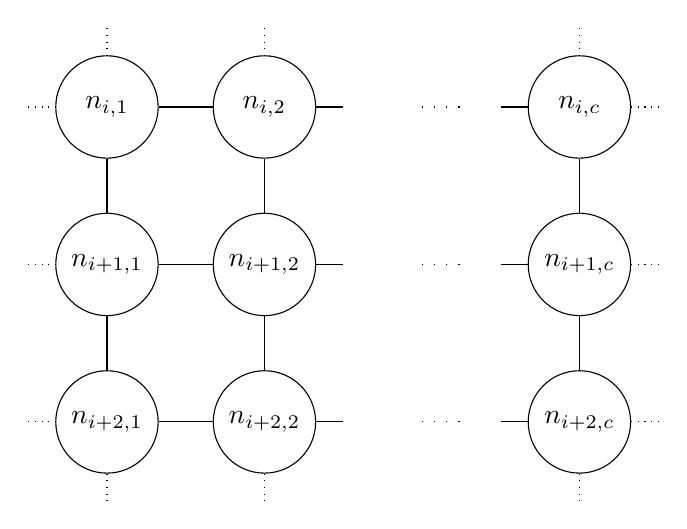
\begin{tikzpicture}[scale=1]
	% Default action for each node
	\tikzstyle{every node}=[draw, shape=circle, minimum size=1.3cm];

	% MIDDLE

										\coordinate (northleft) at (0, 2);		\coordinate (northright) at (2, 2);
	\coordinate (westup) at (-1,1);		\node (r1c1) at (0,1) {$n_{i,1}$};		\node (r1c2) at (2,1) {$n_{i,2}$};		\coordinate (eastup) at (3,1);
	\coordinate (westmid) at (-1,-1);	\node (r2c1) at (0,-1) {$n_{i+1,1}$};	\node (r2c2) at (2,-1) {$n_{i+1,2}$};	\coordinate (eastmid) at (3,-1);
	\coordinate (westdown) at (-1,-3);	\node (r3c1) at (0,-3) {$n_{i+2,1}$};	\node (r3c2) at (2,-3) {$n_{i+2,2}$};	\coordinate (eastdown) at (3,-3);
										\coordinate (southleft) at (0, -4);		\coordinate (southright) at (2, -4);

	% ellipses
	\coordinate (ellipsis westup) at (4,1);		\coordinate (ellipsis eastup) at (4.5,1);
	\coordinate (ellipsis westmid) at (4,-1);	\coordinate (ellipsis eastmid) at (4.5,-1);
	\coordinate (ellipsis westdown) at (4,-3);	\coordinate (ellipsis eastdown) at (4.5,-3);


	% RHS
											\coordinate (rhs north) at (6, 2);
	\coordinate (rhs westup) at (5,1);		\node (r1cn) at (6,1) {$n_{i,c}$};		\coordinate (rhs eastup) at (7,1);
	\coordinate (rhs westmid) at (5,-1);	\node (r2cn) at (6,-1) {$n_{i+1,c}$};	\coordinate (rhs eastmid) at (7,-1);
	\coordinate (rhs westdown) at (5,-3);	\node (r3cn) at (6,-3) {$n_{i+2,c}$};	\coordinate (rhs eastdown) at (7,-3);
											\coordinate (rhs south) at (6, -4);

	% Horizontals
	\draw[outside] (westup) -- (r1c1);
	\draw (r1c1) -- (r1c2);
	\draw (r1c2) -- (eastup);

	\draw[outside] (westmid) -- (r2c1);
	\draw (r2c1) -- (r2c2);
	\draw (r2c2) -- (eastmid);

	\draw[outside] (westdown) -- (r3c1);
	\draw (r3c1) -- (r3c2);
	\draw (r3c2) -- (eastdown);


	\draw[ellipsis] (ellipsis westup) -- (ellipsis eastup);
	\draw[ellipsis] (ellipsis westmid) -- (ellipsis eastmid);
	\draw[ellipsis] (ellipsis westdown) -- (ellipsis eastdown);


	\draw (rhs westup) -- (r1cn);
	\draw[outside] (r1cn) -- (rhs eastup);

	\draw (rhs westmid) -- (r2cn);
	\draw[outside] (r2cn) -- (rhs eastmid);

	\draw (rhs westdown) -- (r3cn);
	\draw[outside] (r3cn) -- (rhs eastdown);

	% Verticals
	\draw[outside] (northleft) -- (r1c1);
	\draw (r1c1) -- (r2c1);
	\draw (r2c1) -- (r3c1);
	\draw[outside] (r3c1) -- (southleft);

	\draw[outside] (northright) -- (r1c2);
	\draw (r1c2) -- (r2c2);
	\draw (r2c2) -- (r3c2);
	\draw[outside] (r3c2) -- (southright);

	\draw[outside] (rhs north) -- (r1cn);
	\draw (r1cn) -- (r2cn);
	\draw (r2cn) -- (r3cn);
	\draw[outside] (r3cn) -- (rhs south);
\end{tikzpicture}



%% Definition B algorithm

\subsection{Algorithm}

\begin{enumerate}
\item Let $n_{i+2,2}$ be the unique vertex in the set $\AdjVV(n_{i+1,2}) \setminus \{ n_{i+1,1} , n_{i+1,3} , n_{i,2} \} $.
\item Let $N = \AdjVV(n_{i+1,1}) \cap \AdjVV(n_{i+2,2})$ be the common neighbours of $n_{i+1,1}$ and $n_{i+2,2}$.
If the number of common neighbours $\card{N}$ is not exactly two, fail the procedure.
\item We know that $n_{i+1,2} \in N$ by construction. Let $n_{i+2,1}$ be the other vertex in $N$.
\item If either of $n_{i+2,1}$ or $n_{i+2,2}$ is in $\Visited$, fail the procedure. Otherwise add the two vertices to $\Visited$.
\item Ensure that the visited neighbours of $n_{i+2,1}$ and $n_{i+2,2}$ are exactly as specified,
that is $n_{i+2,1} \cap \Visited = \{ n_{i+2,2} , n_{i+1,1} \}$ and $n_{i+2,2} \cap \Visited = \{ n_{i+2,1} , n_{i+1,2} \}$.
If this is not the case, remove $n_{i+2,1}$ and $n_{i+2,2}$ from $\Visited$ and fail the procedure.





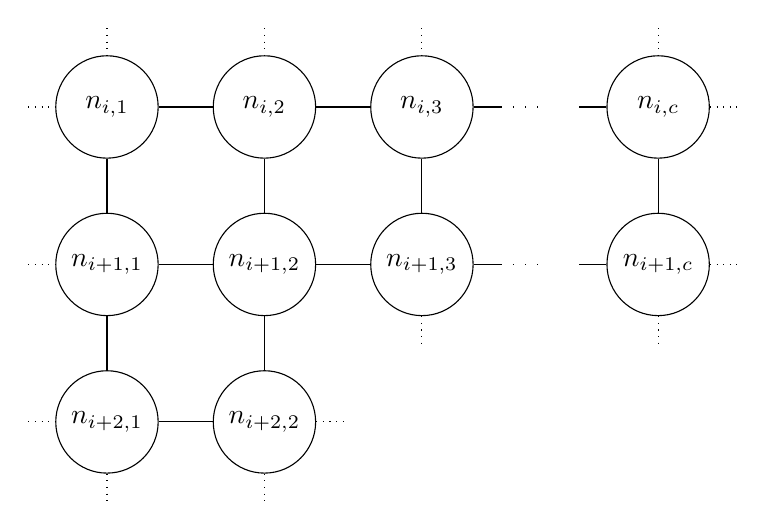
\begin{tikzpicture}[scale=1]
	% Default action for each node
	\tikzstyle{every node}=[draw, shape=circle, minimum size=1.3cm];

	% MIDDLE

										\coordinate (northleft) at (0, 2);		\coordinate (northmid) at (2, 2);		\coordinate (northright) at (4, 2);
	\coordinate (westup) at (-1,1);		\node (r1c1) at (0,1) {$n_{i,1}$};		\node (r1c2) at (2,1) {$n_{i,2}$};		\node (r1c3) at (4,1) {$n_{i,3}$};		\coordinate (eastup) at (5,1);
	\coordinate (westmid) at (-1,-1);	\node (r2c1) at (0,-1) {$n_{i+1,1}$};	\node (r2c2) at (2,-1) {$n_{i+1,2}$};	\node (r2c3) at (4,-1) {$n_{i+1,3}$};	\coordinate (eastmid) at (5,-1);
	\coordinate (westdown) at (-1,-3);	\node (r3c1) at (0,-3) {$n_{i+2,1}$};	\node (r3c2) at (2,-3) {$n_{i+2,2}$};											\coordinate (eastdown) at (3,-3);
										\coordinate (southleft) at (0, -4);		\coordinate (southmid) at (2, -4);		\coordinate (southright) at (4, -2);

	% ellipses
	\coordinate (ellipsis westup) at (5,1);		\coordinate (ellipsis eastup) at (5.5,1);
	\coordinate (ellipsis westdown) at (5,-1);	\coordinate (ellipsis eastdown) at (5.5,-1);


	% RHS
											\coordinate (rhs north) at (7, 2);
	\coordinate (rhs westup) at (6,1);		\node (r1cn) at (7,1) {$n_{i,c}$};		\coordinate (rhs eastup) at (8,1);
	\coordinate (rhs westmid) at (6,-1);	\node (r2cn) at (7,-1) {$n_{i+1,c}$};	\coordinate (rhs eastmid) at (8,-1);
											\coordinate (rhs south) at (7, -2);

	% Horizontals
	\draw[outside] (westup) -- (r1c1);
	\draw (r1c1) -- (r1c2) -- (r1c3) -- (eastup);

	\draw[outside] (westmid) -- (r2c1);
	\draw (r2c1) -- (r2c2) -- (r2c3) -- (eastmid);

	\draw[outside] (westdown) -- (r3c1);
	\draw (r3c1) -- (r3c2);
	\draw[outside] (r3c2) -- (eastdown);


	\draw[ellipsis] (ellipsis westup) -- (ellipsis eastup);
	\draw[ellipsis] (ellipsis westdown) -- (ellipsis eastdown);


	\draw (rhs westup) -- (r1cn);
	\draw[outside] (r1cn) -- (rhs eastup);

	\draw (rhs westmid) -- (r2cn);
	\draw[outside] (r2cn) -- (rhs eastmid);


	% Verticals
	\draw[outside] (northleft) -- (r1c1);
	\draw (r1c1) -- (r2c1);
	\draw (r2c1) -- (r3c1);
	\draw[outside] (r3c1) -- (southleft);

	\draw[outside] (northmid) -- (r1c2);
	\draw (r1c2) -- (r2c2);
	\draw (r2c2) -- (r3c2);
	\draw[outside] (r3c2) -- (southmid);

	\draw[outside] (northright) -- (r1c3);
	\draw (r1c3) -- (r2c3);
	\draw[outside] (r2c3) -- (southright);


	\draw[outside] (rhs north) -- (r1cn);
	\draw (r1cn) -- (r2cn);
	\draw[outside] (r2cn) -- (rhs south);
\end{tikzpicture}




\item For each column\footnote{Possibly none if $c = 3$} $j \in [3..c-1]$:
	\begin{enumerate}
	\item Let $n_{i+2,j}$ be the unique vertex in the set $\AdjVV(n_{i+1,j}) \setminus \{ n_{i+1,j-1} , n_{i+1,j+1} , n_{i,j} \}$.
	\item If $n_{i+2,j} \in \Visited$, remove all vertices in $r_{i+2}$ from $\Visited$, that is $\{ n_{i+2,k} \mid k \in [1..j] \}$ and fail the procedure.
	Otherwise, add $n_{i+2,j}$ $\Visited$.
	\item Ensure that visited neighbours of $n_{i+2,j}$ are exactly $n_{i+2,j-1}$, $n_{i+1,j}$.
	If this is not the case remove vertices $\{ n_{i+2,k} \mid k \in [1..j] \}$ from $\Visited$ and fail the procedure.
	\end{enumerate}




% Foreach j diagram
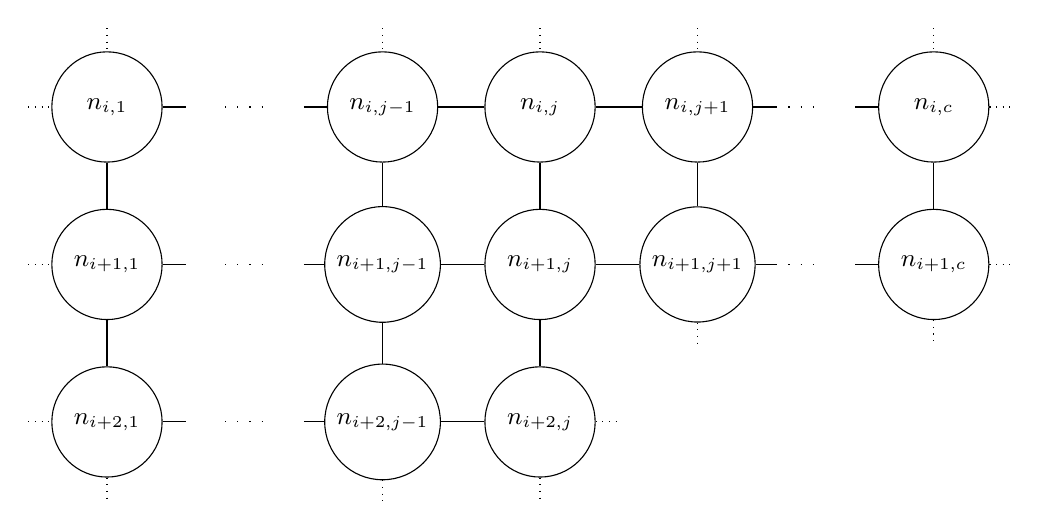
\begin{tikzpicture}[scale=1]
	% Default action for each node
	\tikzstyle{every node}=[draw, shape=circle, minimum size=1.4cm, font=\small];

	% LHS
												\coordinate (lhs north) at (-3.5, 2);
	\coordinate (lhs westup) at (-4.5,1);		\node (r1c0) at (-3.5,1) {$n_{i,1}$};		\coordinate (lhs eastup) at (-2.5,1);
	\coordinate (lhs westmid) at (-4.5,-1);		\node (r2c0) at (-3.5,-1) {$n_{i+1,1}$};	\coordinate (lhs eastmid) at (-2.5,-1);
	\coordinate (lhs westdown) at (-4.5,-3);	\node (r3c0) at (-3.5,-3) {$n_{i+2,1}$};	\coordinate (lhs eastdown) at (-2.5,-3);
												\coordinate (lhs south) at (-3.5, -4);

	% LHS ellipses
	\coordinate (lhs ellipsis westup) at (-2,1);	\coordinate (lhs ellipsis eastup) at (-1.5,1);
	\coordinate (lhs ellipsis westmid) at (-2,-1);	\coordinate (lhs ellipsis eastmid) at (-1.5,-1);
	\coordinate (lhs ellipsis westdown) at (-2,-3);	\coordinate (lhs ellipsis eastdown) at (-1.5,-3);


	% MIDDLE
										\coordinate (northleft) at (0, 2);		\coordinate (northmid) at (2, 2);		\coordinate (northright) at (4, 2);
	\coordinate (westup) at (-1,1);		\node (r1c1) at (0,1) {$n_{i,j-1}$};	\node (r1c2) at (2,1) {$n_{i,j}$};		\node (r1c3) at (4,1) {$n_{i,j+1}$};	\coordinate (eastup) at (5,1);
	\coordinate (westmid) at (-1,-1);	\node (r2c1) at (0,-1) {$n_{i+1,j-1}$};	\node (r2c2) at (2,-1) {$n_{i+1,j}$};	\node (r2c3) at (4,-1) {$n_{i+1,j+1}$};	\coordinate (eastmid) at (5,-1);
	\coordinate (westdown) at (-1,-3);	\node (r3c1) at (0,-3) {$n_{i+2,j-1}$};	\node (r3c2) at (2,-3) {$n_{i+2,j}$};											\coordinate (eastdown) at (3,-3);
										\coordinate (southleft) at (0, -4);		\coordinate (southmid) at (2, -4);		\coordinate (southright) at (4, -2);

	% rhs ellipses
	\coordinate (rhs ellipsis westup) at (5,1);		\coordinate (rhs ellipsis eastup) at (5.5,1);
	\coordinate (rhs ellipsis westdown) at (5,-1);	\coordinate (rhs ellipsis eastdown) at (5.5,-1);


	% RHS
											\coordinate (rhs north) at (7, 2);
	\coordinate (rhs westup) at (6,1);		\node (r1cn) at (7,1) {$n_{i,c}$};		\coordinate (rhs eastup) at (8,1);
	\coordinate (rhs westmid) at (6,-1);	\node (r2cn) at (7,-1) {$n_{i+1,c}$};	\coordinate (rhs eastmid) at (8,-1);
											\coordinate (rhs south) at (7, -2);

	% Horizontals
	\draw[outside] (lhs westup) -- (r1c0);
	\draw (r1c0) -- (lhs eastup);

	\draw[outside] (lhs westmid) -- (r2c0);
	\draw (r2c0) -- (lhs eastmid);

	\draw[outside] (lhs westdown) -- (r3c0);
	\draw (r3c0) -- (lhs eastdown);


	\draw (westup) -- (r1c1) -- (r1c2) -- (r1c3) -- (eastup);

	\draw (westmid) -- (r2c1) -- (r2c2) -- (r2c3) -- (eastmid);

	\draw (westdown) -- (r3c1) -- (r3c2);
	\draw[outside] (r3c2) -- (eastdown);


	\draw[ellipsis] (lhs ellipsis westup) -- (lhs ellipsis eastup);
	\draw[ellipsis] (lhs ellipsis westmid) -- (lhs ellipsis eastmid);
	\draw[ellipsis] (lhs ellipsis westdown) -- (lhs ellipsis eastdown);

	\draw[ellipsis] (rhs ellipsis westup) -- (rhs ellipsis eastup);
	\draw[ellipsis] (rhs ellipsis westdown) -- (rhs ellipsis eastdown);


	\draw (rhs westup) -- (r1cn);
	\draw[outside] (r1cn) -- (rhs eastup);

	\draw (rhs westmid) -- (r2cn);
	\draw[outside] (r2cn) -- (rhs eastmid);


	% Verticals
	\draw[outside] (lhs north) -- (r1c0);
	\draw (r1c0) -- (r2c0) -- (r3c0);
	\draw[outside] (r3c0) -- (lhs south);


	\draw[outside] (northleft) -- (r1c1);
	\draw (r1c1) -- (r2c1) -- (r3c1);
	\draw[outside] (r3c1) -- (southleft);

	\draw[outside] (northmid) -- (r1c2);
	\draw (r1c2) -- (r2c2) -- (r3c2);
	\draw[outside] (r3c2) -- (southmid);

	\draw[outside] (northright) -- (r1c3);
	\draw (r1c3) -- (r2c3);
	\draw[outside] (r2c3) -- (southright);


	\draw[outside] (rhs north) -- (r1cn);
	\draw (r1cn) -- (r2cn);
	\draw[outside] (r2cn) -- (rhs south);
\end{tikzpicture}







\item Consider $\AdjVV(n_{i+2,c-1}) \cap \AdjVV(n_{i+1,c})$, the common neighbours of $n_{i+2,c-1}$ and $n_{i+1,c}$.
If these are not exactly two neighbours, remove vertices $\{ n_{i+2,k} \mid k \in [1..c-1] \}$ from $\Visited$ and fail the procedure.
\item One of the two neighbours must be $n_{i+1,c}$ by construction. Let $n_{i+2,c}$ denote the other neighbour.
\item If $n_{i+2,c} \in \Visited$, remove vertices $\{ n_{i+2,k} \mid k \in [1..c-1] \}$ from $\Visited$ and fail the procedure.
Otherwise, add $n_{i+2,c}$ to $\Visited$.
\item Ensure that the visited neighbours of $n_{i+2,c}$ are exactly $\{ n_{i+2,c-1} , n_{i+1,c} \}$,
that is $\AdjVV(n_{i+2,c}) \cap \Visited = \{ n_{i+2,c-1} , n_{i+1,c} \}$. If this is not the case remove vertices $\{ n_{i+2,k} \mid k \in [1..c] \}$ from $\Visited$ and fail the procedure.




% lastnode diagram
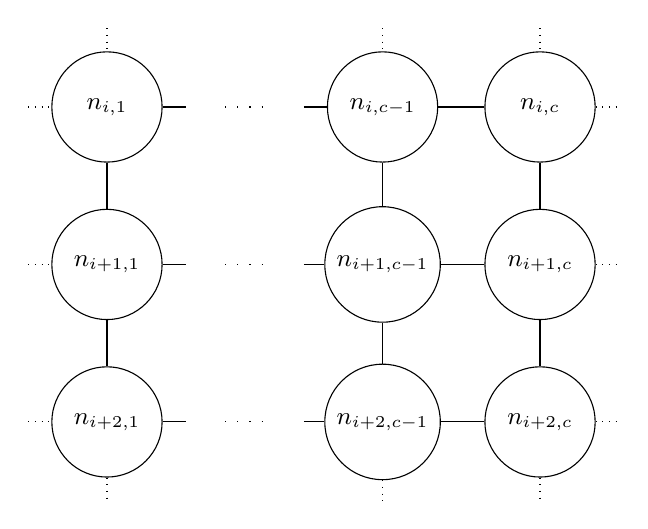
\begin{tikzpicture}[scale=1]
	% Default action for each node
	\tikzstyle{every node}=[draw, shape=circle, minimum size=1.4cm, font=\small];

	% LHS
												\coordinate (lhs north) at (-1.5, 2);
	\coordinate (lhs westup) at (-2.5,1);		\node (r1c0) at (-1.5,1) {$n_{i,1}$};		\coordinate (lhs eastup) at (-0.5,1);
	\coordinate (lhs westmid) at (-2.5,-1);		\node (r2c0) at (-1.5,-1) {$n_{i+1,1}$};	\coordinate (lhs eastmid) at (-0.5,-1);
	\coordinate (lhs westdown) at (-2.5,-3);	\node (r3c0) at (-1.5,-3) {$n_{i+2,1}$};	\coordinate (lhs eastdown) at (-0.5,-3);
												\coordinate (lhs south) at (-1.5, -4);

	% LHS ellipses
	\coordinate (lhs ellipsis westup) at (0,1);		\coordinate (lhs ellipsis eastup) at (0.5,1);
	\coordinate (lhs ellipsis westmid) at (0,-1);	\coordinate (lhs ellipsis eastmid) at (0.5,-1);
	\coordinate (lhs ellipsis westdown) at (0,-3);	\coordinate (lhs ellipsis eastdown) at (0.5,-3);


	% MIDDLE
										\coordinate (northmid) at (2, 2);		\coordinate (northright) at (4, 2);
	\coordinate (westup) at (1,1);		\node (r1c2) at (2,1) {$n_{i,c-1}$};	\node (r1c3) at (4,1) {$n_{i,c}$};		\coordinate (eastup) at (5,1);
	\coordinate (westmid) at (1,-1);	\node (r2c2) at (2,-1) {$n_{i+1,c-1}$};	\node (r2c3) at (4,-1) {$n_{i+1,c}$};	\coordinate (eastmid) at (5,-1);
	\coordinate (westdown) at (1,-3);	\node (r3c2) at (2,-3) {$n_{i+2,c-1}$};	\node (r3c3) at (4,-3) {$n_{i+2,c}$};	\coordinate (eastdown) at (5,-3);
										\coordinate (southmid) at (2, -4);		\coordinate (southright) at (4, -4);




	% Horizontals
	\draw[outside] (lhs westup) -- (r1c0);
	\draw (r1c0) -- (lhs eastup);

	\draw[outside] (lhs westmid) -- (r2c0);
	\draw (r2c0) -- (lhs eastmid);

	\draw[outside] (lhs westdown) -- (r3c0);
	\draw (r3c0) -- (lhs eastdown);


	\draw (westup) -- (r1c2) -- (r1c3);
	\draw[outside] (r1c3) -- (eastup);

	\draw (westmid) -- (r2c2) -- (r2c3);
	\draw[outside] (r2c3) -- (eastmid);

	\draw (westdown) -- (r3c2) -- (r3c3);
	\draw[outside] (r3c3) -- (eastdown);


	\draw[ellipsis] (lhs ellipsis westup) -- (lhs ellipsis eastup);
	\draw[ellipsis] (lhs ellipsis westmid) -- (lhs ellipsis eastmid);
	\draw[ellipsis] (lhs ellipsis westdown) -- (lhs ellipsis eastdown);


	% Verticals
	\draw[outside] (lhs north) -- (r1c0);
	\draw (r1c0) -- (r2c0) -- (r3c0);
	\draw[outside] (r3c0) -- (lhs south);

	\draw[outside] (northmid) -- (r1c2);
	\draw (r1c2) -- (r2c2) -- (r3c2);
	\draw[outside] (r3c2) -- (southmid);

	\draw[outside] (northright) -- (r1c3);
	\draw (r1c3) -- (r2c3) -- (r3c3);
	\draw[outside] (r3c3) -- (southright);

\end{tikzpicture}

\item Return the vertices of node row $r_{i+2}$, that is $n_{i+2,1} \cdots n_{i+2,c}$.
\end{enumerate}





%%%% PHASE 3

\section{Phase 3: Extend rows}
%% Phase 3.1 summary
``Extend a row'' is iteratively applied, starting from $r_1 = n_{1,1} \cdots n_{1,c}$ and $r_2 = n_{2,1} \cdots n_{2,c}$, to yield successive rows until it fails.
The resulting rows are appended \emph{below} $\Structured$.


%% Phase 3.1 diagram
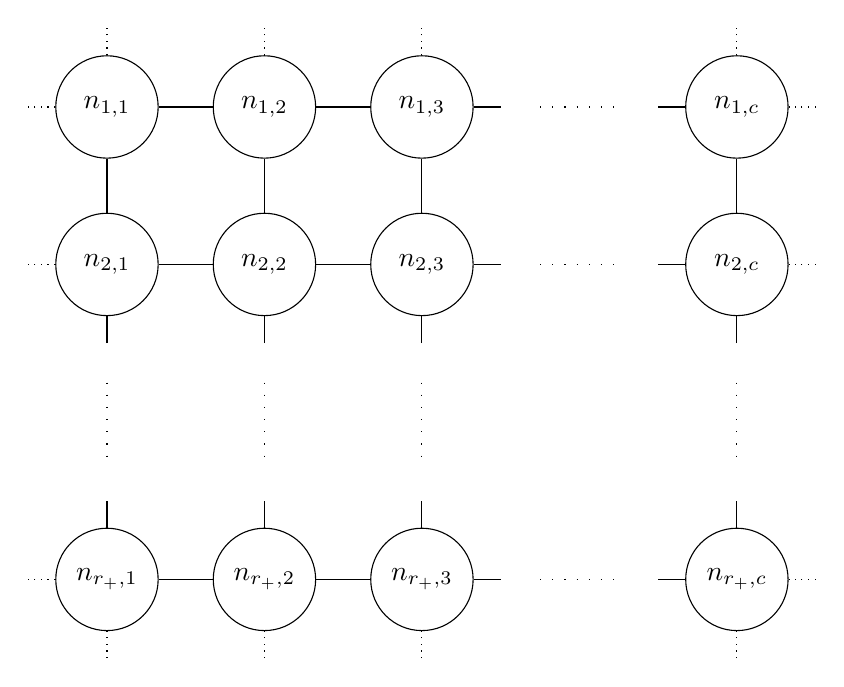
\begin{tikzpicture}
	\tikzstyle{every node}=[draw, shape=circle, minimum size=1.3cm];

	% First rows
	\drawellipsiscol{num=2, rowoffset=6, coloffset=7.5}
	\drawgrid{rows=2, cols=3, rowoffset=6,
		labeler=\plainlabelnode, labelerA=0, labelerB=0,
		southborder=structured, eastborder=structured}
	\drawgrid{rows=2, cols=1, rowoffset=6, coloffset=8,
		labeler=\varcollabelnode, labelerA=0, labelerB=0, labelerC=c,
		southborder=structured, westborder=structured}

	% Bottom horizontal ellipsis
	\drawellipsisrow{num=3, rowoffset=0.5}
	\drawellipsisrow{num=1, rowoffset=0.5, coloffset=8}

	% Last row
	\drawellipsiscol{num=1, rowoffset=0, coloffset=7.5}
	\drawgrid{rows=1, cols=3, rowoffset=0,
		labeler=\varrowlabelnode, labelerA=0, labelerB=0, labelerC=r_+,
		northborder=structured, eastborder=structured}
	\drawgrid{rows=1, cols=1, rowoffset=0, coloffset=8,
		labeler=\varlabelnode, labelerA=0, labelerB=0, labelerC=r_+, labelerD=c,
		northborder=structured, westborder=structured}
\end{tikzpicture}




%% Phase 3.2 summary
``Extend a row'' is iteratively applied, starting from the mirror image of the initial rows about the x-axis, that is $r_1 = n_{2,1} \cdots n_{2,c}$ and $r_2 = n_{1,1} \cdots n_{1,c}$, to yield successive rows until it fails.
The resulting rows are appended \emph{above} $\Structured$.

%% Phase 3.2 diagram
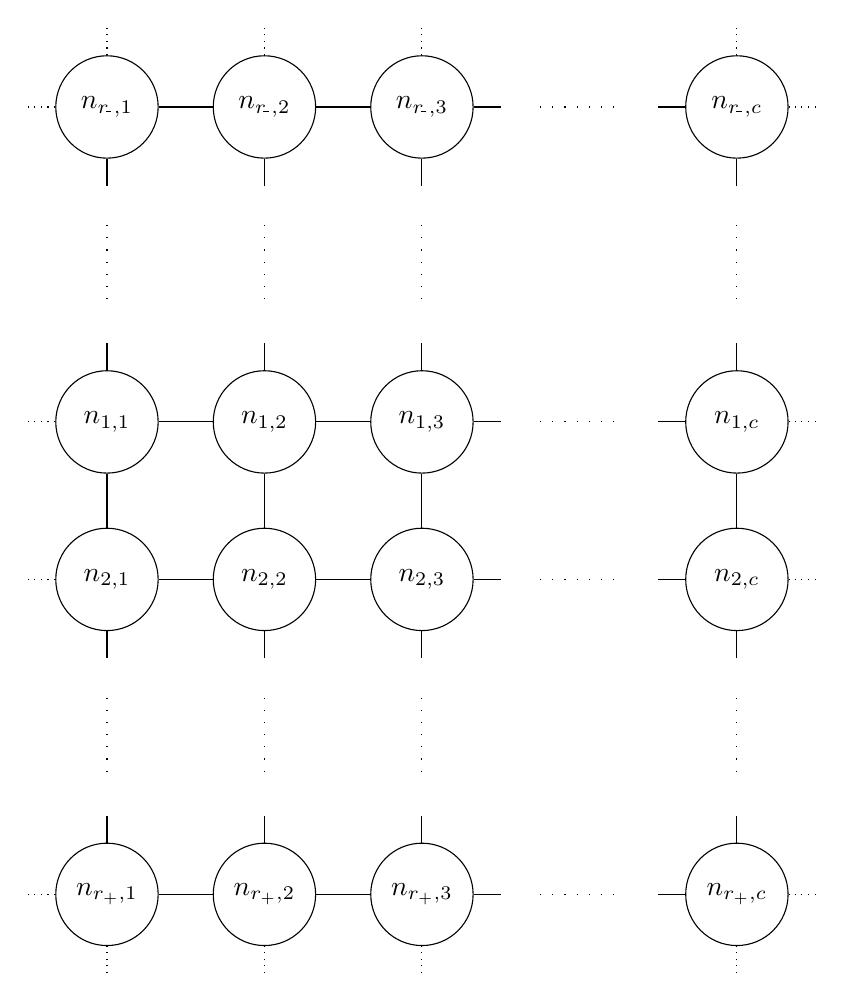
\begin{tikzpicture}
	\tikzstyle{every node}=[draw, shape=circle, minimum size=1.3cm];

	% First first rows
	\drawellipsiscol{num=1, rowoffset=10, coloffset=7.5}
	\drawgrid{rows=1, cols=3, rowoffset=10,
		labeler=\varrowlabelnode, labelerA=0, labelerB=0, labelerC=r_{\!^{\_}},
		southborder=structured, eastborder=structured}
	\drawgrid{rows=1, cols=1, rowoffset=10, coloffset=8,
		labeler=\varlabelnode, labelerA=0, labelerB=0, labelerC=r_{\!^{\_}}, labelerD=c,
		southborder=structured, westborder=structured}

	% Top horizontal ellipsis
	\drawellipsisrow{num=3, rowoffset=6.5}
	\drawellipsisrow{num=1, rowoffset=6.5, coloffset=8}

	% First rows
	\drawellipsiscol{num=2, rowoffset=6, coloffset=7.5}
	\drawgrid{rows=2, cols=3, rowoffset=6,
		labeler=\plainlabelnode, labelerA=0, labelerB=0,
		southborder=structured, eastborder=structured, northborder=structured}
	\drawgrid{rows=2, cols=1, rowoffset=6, coloffset=8,
		labeler=\varcollabelnode, labelerA=0, labelerB=0, labelerC=c,
		southborder=structured, westborder=structured, northborder=structured}

	% Bottom horizontal ellipsis
	\drawellipsisrow{num=3, rowoffset=0.5}
	\drawellipsisrow{num=1, rowoffset=0.5, coloffset=8}

	% Last row
	\drawellipsiscol{num=1, rowoffset=0, coloffset=7.5}
	\drawgrid{rows=1, cols=3, rowoffset=0,
		labeler=\varrowlabelnode, labelerA=0, labelerB=0, labelerC=r_+,
		northborder=structured, eastborder=structured}
	\drawgrid{rows=1, cols=1, rowoffset=0, coloffset=8,
		labeler=\varlabelnode, labelerA=0, labelerB=0, labelerC=r_+, labelerD=c,
		northborder=structured, westborder=structured}
\end{tikzpicture}


%% Phase 3 algorithm

\subsection{Algorithm}

\paragraph{Extend below}
\begin{enumerate}
\item Let $r_a = n_{1,1} \cdots n_{1,c}$ and $r_b = n_{2,1} \cdots n_{2,c}$ be the first two structured node rows.
\item \label{step:extend_row} Let $n_{i,1} \cdots n_{i,c}$ and $n_{i+1,1} \cdots n_{i+1,c}$ represent the respective elements of $r_a$ and $r_b$.
\item Call the procedure ``Extend a row'' with $r_a$ and $r_b$ as inputs.
\item If the procedure fails, go to step~\ref{step:init_reverse_row}.
\item Otherwise, append the new row obtained $r_{new} = n_{i+2,1} \cdots n_{i+2,c}$ \emph{below} $\Structured$.\\
Thus $\Structured$ will become:
$\begin{bmatrix}
	n_{1,1}   & n_{1,2}   & \cdots  & n_{1,c}   \\
	n_{2,1}   & n_{2,2}   & \cdots  & n_{2,c}   \\
	\vdots    & \vdots    &         & \vdots    \\
	n_{i,1}   & n_{i,2}   & \cdots  & n_{i,c}   \\
	n_{i+1,1} & n_{i+1,2} & \cdots  & n_{i+1,c} \\
	n_{i+2,1} & n_{i+2,2} & \cdots  & n_{i+2,c}
	\end{bmatrix}$
\item Set $r_a = n_{i+1,1} \cdots n_{i+1,c}$ and $r_b = n_{i+2,1} \cdots n_{i+2,c}$, and continue from step~\ref{step:extend_row}.
\end{enumerate}

\paragraph{Extend above}
\begin{enumerate}[resume]
\item \label{step:init_reverse_row} Let $r_a = n_{2,1} \cdots n_{2,c}$ and $r_b = n_{1,1} \cdots n_{1,c}$ be the first two structured node rows, the other way around.
\item \label{step:reverse_extend_row} Let $n_{i,1} \cdots n_{i,c}$ and $n_{i+1,1} \cdots n_{i+1,c}$ represent the respective elements of $r_a$ and $r_b$.
\item Call the procedure ``Extend a row'' with $r_a$ and $r_b$ as inputs.
\item If the procedure fails, return immediately.
\item Otherwise, append the new row obtained $r_{new} = n_{i+2,1} \cdots n_{i+2,c}$ \emph{above} $\Structured$.\\
Thus $\Structured$ will become:
$\begin{bmatrix}
	n_{i+2,1} & n_{i+2,2} & \cdots  & n_{i+2,c} \\
	n_{i+1,1} & n_{i+1,2} & \cdots  & n_{i+1,c} \\
	n_{i,1}   & n_{i,2}   & \cdots  & n_{i,c}   \\
	\vdots    & \vdots    &         & \vdots    \\
	n_{1,1}   & n_{1,2}   & \cdots  & n_{1,c}   \\
	n_{2,1}   & n_{2,2}   & \cdots  & n_{2,c}   \\
	\vdots    & \vdots    &         & \vdots    \\
	n_{r_+,1} & n_{r_+,2} & \cdots  & n_{r_+,c}
	\end{bmatrix}$
\item Set $r_a = n_{i+1,1} \cdots n_{i+1,c}$ and $r_b = n_{i+2,1} \cdots n_{i+2,c}$, and continue from step~\ref{step:reverse_extend_row}.
\end{enumerate}

\section{Sketch proof of complexity analysis}
We argue that the length-first search algorithm presented in this chapter runs in $O(\Structured)$, that is linear in the size of the detected structured region\footnote{If no structured region is detected, then we take this to mean that the run-time should be constant, $O(1)$.}.

Neighbour queries are performed using the relation-maps available, and are hence assumed to run in $O(1)$. Set operations such as set-intersection and set-difference between a constant neighbours also run in $O(1)$, as we assume some (again small) constant upper bound on the number of neighbours.

Querying the visited set or adding a vertex to it is done in $O(1)$.

If the algorithm terminates having not found any structure region, which can only occur in the \emph{grow a quad} phase, then it would have only examined a constant number of neighbours and applied a constant number of set-operations.

If the algorithm terminates having found a structured region, then it must have called the ``extend a quad'' and ``extend rows'' functions a number of times linear in $\Structured$. We know this since each call to those functions adds a new vertex to $\Structured$. All other remaining work performed is linear in time.

Thus the time complexity of the length-first search algorithm is $O(\Structured)$.

\subsection{A corollary}
Given that length-first search runs in $O(\Structured)$, we show that using it for detecting multiple structure regions results in an $O(\VertexSet)$ time complexity.

For every application of length-first search, we detect $\Structured$ vertices in $O(\Structured)$ time. Vertices which are detected are added to the visited set and hence are not used as a starting vertex in the future. Since length-first search consumes as many vertices as it consumes time (asymptotically speaking), then by the end we would have exhausted all vertices, and have done so in $O(\VertexSet$).

\section{Chapter summary}
In this chapter we refined our sketch of the length-first search algorithm into a more precise form more amenable for complexity analysis. On this basis we analyse the algorithmic complexity of the algorithm, and find it to be linear in the number of vertices.

\chapter{Evaluation}
\begin{figure}[h]
  \centering
  \begin{tikzpicture}
\begin{axis}[
xbar,
flexible yticklabels from table={data-airfoil-numbering.tsv}{category}{},
y tick label style={rotate=45, anchor=north east},
ytick=data,
ylabel = Renumbering applied,
xlabel = Core-computation runtime (s),
legend pos = south east
]


\addplot [
draw=blue,
pattern=horizontal lines light blue
] table [
y expr=\coordindex,
x = baseline
] {data-airfoil-numbering.tsv};


\addlegendentry{Baseline run};

\addplot [
draw=black,
pattern=horizontal lines dark blue
] table [
y expr=\coordindex,
x = mine
] {data-airfoil-numbering.tsv};

\addlegendentry{Crystal run};

\end{axis}
\end{tikzpicture}

\caption{Impact of renumbering}
\label{fig:plot-airfoil-numbering}
\end{figure}


\begin{figure}[h]
  \centering
  \begin{tikzpicture}
\begin{axis}[
xlabel = Mesh size,
ylabel = Core-computation runtime (s),
legend pos = north west
]


\addplot [
draw=blue,
mark = x,
] table [
y = baseline
] {data-airfoil-size.tsv};


\addlegendentry{Baseline run};

\addplot [
draw=black,
mark = triangle,
] table [
y = mine
] {data-airfoil-size.tsv};

\addlegendentry{Crystal run};

\addplot [
draw=red,
mark = square,
] table [
y = {detection time}
] {data-airfoil-size.tsv};

\addlegendentry{Detection time};

\end{axis}
\end{tikzpicture}

\caption{Impact of mesh size}
\label{fig:plot-airfoil-size-runtime}
\end{figure}


\begin{figure}[h]
  \centering
  \begin{tikzpicture}
\begin{axis}[
xlabel = Number of iterations,
ylabel = Total runtime (s),
xmax = 2000,
legend pos = north west
]


\addplot [
draw=blue,
mark = x,
] table [
y = baselinetime
] {data-airfoil-iterations.tsv};


\addlegendentry{Baseline run};

\addplot [
draw=black,
mark = triangle,
] table [
y = mytime
] {data-airfoil-iterations.tsv};

\addlegendentry{Crystal run};

\end{axis}
\end{tikzpicture}

\caption{Number of airfoil iterations needed to overcome structure detection cost}
\label{fig:plot-airfoil-iterations}
\end{figure}



\section{Structure detection}



\nocite{*} % Show all Bib-entries
\bibliographystyle{plain}
\bibliography{thesis}

\end{document}
